% ============================================================
%  TD4 – Exploración, Limpieza y Selección de Características
%  Curso: Machine Learning Industrial – Detección de Fallos
% ============================================================
\documentclass[12pt,a4paper]{article}

% ---- Paquetes ----
\usepackage[a4paper, top=2.5cm, bottom=2.5cm, left=2.8cm, right=2.8cm, headheight=14pt]{geometry}
\usepackage[spanish]{babel}
\usepackage[T1]{fontenc}
\usepackage[utf8]{inputenc}
\usepackage{amsmath, amssymb}
\usepackage{booktabs}
\usepackage{graphicx}
\usepackage{float}
\usepackage{xcolor}
\usepackage{listings}
\usepackage{hyperref}
\usepackage{parskip}
\usepackage{titlesec}
\usepackage{enumitem}
\usepackage{array}
\usepackage{multirow}
\usepackage{fancyhdr}
\usepackage{tcolorbox}
\usepackage{subcaption}

% ---- Ruta de imágenes ----
\graphicspath{{img/}}

% ---- Colores ----
\definecolor{myblue}{RGB}{0,70,140}
\definecolor{mygreen}{RGB}{0,128,64}
\definecolor{mygray}{RGB}{245,245,245}
\definecolor{myorange}{RGB}{200,80,0}
\definecolor{codebg}{RGB}{248,248,248}
\definecolor{codeframe}{RGB}{180,180,180}
\definecolor{keywordcolor}{RGB}{0,0,180}
\definecolor{commentcolor}{RGB}{80,120,80}
\definecolor{stringcolor}{RGB}{160,32,32}
\definecolor{whyblue}{RGB}{0,50,120}

% ---- Estilo de código Python ----
\lstset{
  language=Python,
  basicstyle=\small\ttfamily,
  keywordstyle=\color{keywordcolor}\bfseries,
  commentstyle=\color{commentcolor}\itshape,
  stringstyle=\color{stringcolor},
  numberstyle=\tiny\color{gray},
  backgroundcolor=\color{codebg},
  frame=single,
  rulecolor=\color{codeframe},
  numbers=left,
  numbersep=8pt,
  breaklines=true,
  breakatwhitespace=false,
  showstringspaces=false,
  tabsize=4,
  captionpos=b,
  xleftmargin=15pt,
  xrightmargin=5pt,
  aboveskip=8pt,
  belowskip=8pt,
}

% ---- Formato de secciones ----
\titleformat{\section}[block]
  {\large\bfseries\color{myblue}}
  {\thesection.}{0.6em}{}[\vspace{2pt}\titlerule]

\titleformat{\subsection}[block]
  {\normalsize\bfseries\color{myblue!80!black}}
  {\thesubsection.}{0.5em}{}

\titleformat{\subsubsection}[block]
  {\normalsize\bfseries\color{myorange}}
  {\thesubsubsection.}{0.5em}{}

% ---- Encabezado y pie ----
\pagestyle{fancy}
\fancyhf{}
\renewcommand{\headrulewidth}{0.4pt}
\fancyhead[L]{\small\textcolor{myblue}{TD4 – Machine Learning Industrial}}
\fancyhead[R]{\small\textcolor{myblue}{Detección de Fallos en Motores}}
\fancyfoot[C]{\small\thepage}

% ---- Cajas de contenido ----
\tcbuselibrary{skins,breakable}
\newtcolorbox{notebox}{
  colback=myblue!5,
  colframe=myblue!50,
  fonttitle=\bfseries,
  title=Nota Clave,
  breakable
}
\newtcolorbox{resultbox}{
  colback=mygreen!5,
  colframe=mygreen!50,
  fonttitle=\bfseries,
  title=Resultado,
  breakable
}
\newtcolorbox{warningbox}{
  colback=myorange!5,
  colframe=myorange!50,
  fonttitle=\bfseries,
  title=Precaución,
  breakable
}
\newtcolorbox{whybox}{
  colback=whyblue!5,
  colframe=whyblue!40,
  fonttitle=\bfseries\color{whyblue},
  title={Por que este paso?},
  breakable
}

% ============================================================
\begin{document}

% ---- PORTADA ----
\begin{titlepage}
  \thispagestyle{empty}
  \begin{center}
    \vspace*{1.5cm}
    {\LARGE\bfseries\color{myblue}
      TD4: Exploración, Limpieza\\[0.3em]
      y Selección de Características}\\[1.2em]
    \rule{0.8\linewidth}{1.5pt}\\[0.8em]
    {\large\itshape Data Challenge Kaggle –
      Detección de Fallos en Motores Servo-Robóticos}\\[2em]

    \begin{tcolorbox}[colback=mygray, colframe=myblue!40, width=0.85\linewidth]
      \centering
      \textbf{Descripción del Proyecto}\\[0.5em]
      Sistema de 6 motores servo-robóticos monitoreados con 3 señales cada uno
      (posición, temperatura, voltaje). El objetivo es construir un pipeline
      completo de preprocesamiento y selección de características para la
      detección automática de fallos en el marco de un desafío de datos
      en Kaggle.
    \end{tcolorbox}

    \vfill
    \begin{tabular}{ll}
      \textbf{Curso:}      & Machine Learning Industrial\\
      \textbf{Tarea:}      & TD4 – Preprocesamiento y Feature Engineering\\
      \textbf{Frecuencia:} & $\approx 10\,\text{Hz}$ (muestras cada 0.1 s)\\
      \textbf{Dataset:}    & 39.309 filas $\times$ 26 columnas, 23 secuencias\\
      \textbf{Fecha:}      & Junio 2026\\
    \end{tabular}
  \end{center}
\end{titlepage}

% ---- RESUMEN EJECUTIVO ----
\section*{Resumen Ejecutivo}
\addcontentsline{toc}{section}{Resumen Ejecutivo}

Este documento describe en detalle la metodología, decisiones técnicas y resultados
obtenidos en el TD4 del curso de Machine Learning Industrial.
El trabajo se organiza en tres tareas principales:

\begin{enumerate}[leftmargin=2em]
  \item \textbf{Task 1 – Lectura y comprensión de datos:} carga del dataset, análisis
    estadístico exploratorio (histogramas, boxplots) e inspección visual de las señales
    temporales; finalizando con un análisis de componentes principales (PCA) para
    entender la estructura dimensional de los datos.

  \item \textbf{Task 2 – Limpieza y preprocesamiento:} normalización con
    \texttt{StandardScaler}, eliminación de outliers mediante recorte por rango físico
    y z-score, y suavizado temporal con media móvil causal.

  \item \textbf{Task 3 – Ingeniería de características:} violin plots para medir poder
    discriminativo, matriz de correlación de Pearson para detectar redundancias,
    y recomendaciones finales de selección de características.
\end{enumerate}

Al término del pipeline, se eliminaron \textbf{6.840 outliers} (0.97\% de los valores
de características), se redujo la dimensionalidad de 18 señales brutas a un subconjunto
recomendado de \textbf{10 características} de alta relevancia, y se documentaron las
limitaciones clave del dataset (desequilibrio de clases, concentración de fallos en
una sola sesión).

\tableofcontents
\newpage

% ============================================================
\section{Contexto y Descripción del Dataset}

\subsection{El Sistema Físico}

El dataset proviene de un banco de pruebas de 6 motores servo-robóticos idénticos
que operan en paralelo. Cada motor puede encontrarse en dos estados:
\textbf{normal} (etiqueta 0) o \textbf{fallo} (etiqueta 1).
Los fallos son inducidos deliberadamente en experimentos controlados para generar
datos de entrenamiento.

Cada motor es monitorizado con tres tipos de señales:

\begin{table}[H]
\centering
\caption{Descripción de señales por motor}
\begin{tabular}{@{}llll@{}}
\toprule
\textbf{Señal} & \textbf{Unidad} & \textbf{Rango físico} & \textbf{Descripción}\\
\midrule
Posición    & encoder (u.a.) & [0, 1000]       & Ángulo/posición del eje, varía entre dos set-points\\
Temperatura & °C             & [0, 100]        & Temperatura de la bobina/carcasa del motor\\
Voltaje     & mV             & [6000, 9000]    & Tensión de alimentación registrada por el driver\\
\bottomrule
\end{tabular}
\end{table}

La frecuencia de muestreo es de \textbf{10 Hz} (una muestra cada 0.1 s), suficiente
para capturar dinámicas térmicas lentas y variaciones de posición durante movimientos
robóticos. La duración de cada secuencia de test varía entre aproximadamente 70 s
(las más cortas) y 350 s (las más largas).

\subsection{Estructura del Dataset}

El dataset se carga con la función \texttt{read\_all\_test\_data\_from\_path} definida
en \texttt{utility.py}, que concatena todos los archivos CSV de una carpeta en un único
DataFrame de pandas.

\begin{lstlisting}[caption={Carga del dataset completo}, label={lst:load}]
from utility import read_all_test_data_from_path

DATA_PATH = "./data/"
df = read_all_test_data_from_path(DATA_PATH)
print(df.shape)          # (39309, 26)
print(df.dtypes)
print(df.head())
\end{lstlisting}

El DataFrame resultante tiene \textbf{39.309 filas} y \textbf{26 columnas}, distribuidas
de la siguiente manera:

\begin{itemize}[leftmargin=2em]
  \item \texttt{time} – marca temporal en segundos (float64)
  \item Para cada motor $i \in \{1, 2, 3, 4, 5, 6\}$:
    \begin{itemize}
      \item \texttt{data\_motor\_\textit{i}\_position} – posición del encoder
      \item \texttt{data\_motor\_\textit{i}\_temperature} – temperatura en °C
      \item \texttt{data\_motor\_\textit{i}\_voltage} – voltaje en mV
      \item \texttt{data\_motor\_\textit{i}\_label} – etiqueta binaria (0=normal, 1=fallo)
    \end{itemize}
  \item \texttt{test\_condition} – identificador de la secuencia de test (timestamp)
\end{itemize}

\begin{lstlisting}[caption={Inspección de columnas y tipos}, label={lst:cols}]
# Columnas del DataFrame
print(df.columns.tolist())
# ['time', 'data_motor_1_position', 'data_motor_1_temperature',
#  'data_motor_1_voltage', 'data_motor_1_label', ...,
#  'data_motor_6_label', 'test_condition']

# Identificar secuencias de test
sequences = df['test_condition'].unique()
print(f"Numero de secuencias: {len(sequences)}")   # 23
print(sequences[:3])
# ['20240105_164214', '20240107_153012', ...]
\end{lstlisting}

\subsection{Distribución de Etiquetas (Tasa de Fallos)}

El dataset es \textbf{fuertemente desequilibrado}. La tabla siguiente muestra
el porcentaje de muestras con etiqueta de fallo para cada motor:

\begin{table}[H]
\centering
\caption{Tasa de fallos por motor}
\begin{tabular}{@{}lcc@{}}
\toprule
\textbf{Motor} & \textbf{Muestras con fallo} & \textbf{Tasa (\%)}\\
\midrule
Motor 1 & $\sim 1\,600$  & $\approx 4.1\%$\\
Motor 2 & $\sim 6\,700$  & $\approx 17.0\%$\\
Motor 3 & $< 200$        & $< 0.5\%$\\
Motor 4 & $\sim 6\,700$  & $\approx 17.0\%$\\
Motor 5 & $< 200$        & $< 0.5\%$\\
Motor 6 & $\sim 2\,000$  & $\approx 5.1\%$\\
\bottomrule
\end{tabular}
\end{table}

\begin{warningbox}
Los motores 3 y 5 tienen menos del 0.5\% de muestras de fallo. Con tan pocos ejemplos
positivos, los clasificadores estándar de dos clases tenderán a ignorar la clase
minoritaria. Para estos motores se recomienda explorar técnicas de detección de
anomalías (one-class SVM, Isolation Forest, autoencoders) en lugar de clasificación
binaria clásica.

Adicionalmente, la mayor parte de los fallos de los motores 2 y 4 provienen de una
\textbf{única sesión de test}: \texttt{20240325\_155003}. Esta concentración introduce
el riesgo de que el modelo aprenda características de esa sesión específica en lugar
del fallo en sí.
\end{warningbox}

% ============================================================
\section{Task 1: Lectura y Comprensión de Datos}

\subsection{Sub-tarea 1: Carga y Estadísticas Descriptivas}

\begin{whybox}
\textbf{Objetivo de este paso:} Antes de realizar cualquier transformación, es
imprescindible establecer una línea base del estado del dataset: ¿hay valores
nulos? ¿Los tipos de datos son correctos? ¿Las escalas tienen sentido físico?

\textbf{Por qué primero estadísticas descriptivas y no visualizaciones:}
Las estadísticas descriptivas (media, desviación estándar, mínimo, máximo,
percentiles) son computacionalmente baratas y responden de forma objetiva y
cuantitativa a las preguntas fundamentales de calidad de datos. La visualización
viene después para confirmar y matizar lo que los números ya sugieren. En particular,
los valores extremos de mínimo y máximo ya revelan outliers potenciales antes de
dibujar un solo histograma.

\textbf{Alternativa descartada:} Empezar directamente con modelos sin exploración
previa (``black-box pipeline'') es un error común. Si el dataset tiene valores de
temperatura de 255 °C sin ser detectados, el modelo los aprenderá como señal válida,
degradando el rendimiento de forma invisible.
\end{whybox}

El primer paso es verificar la integridad del dataset: dimensiones, tipos de datos,
presencia de valores nulos y rango de cada variable.

\begin{lstlisting}[caption={Estadísticas descriptivas básicas}, label={lst:describe}]
print("Shape:", df.shape)                  # (39309, 26)
print("\nNulos por columna:")
print(df.isnull().sum())                   # 0 en todas las columnas

# Estadisticas descriptivas
print(df.describe().T)

# Verificar secuencias
n_seq = df['test_condition'].nunique()     # 23
seq_lengths = df.groupby('test_condition').size()
print(seq_lengths.describe())
# min~700, max~3500, mean~1709
\end{lstlisting}

\begin{resultbox}
El dataset no contiene valores nulos en su forma original. Todos los tipos son
numéricos (\texttt{float64} para señales, \texttt{int64} para etiquetas).
Las 23 secuencias tienen longitudes variables entre aproximadamente 700 y 3.500
muestras, lo que refleja duraciones de experimento distintas.

Sin embargo, las estadísticas de mínimo/máximo revelan señales de alarma:
el máximo de temperatura en algunos motores supera los 200 °C, lo que es
físicamente imposible para este tipo de servo y sugiere saturación del sensor ADC.
\end{resultbox}

\subsection{Sub-tarea 2: Visualización de Señales Temporales Crudas}

\begin{whybox}
\textbf{Por qué visualizar las señales crudas antes de procesar:}
La inspección visual de las series temporales permite identificar patrones
que las estadísticas resumen no capturan:
\begin{itemize}[leftmargin=1.5em]
  \item Presencia de transitorios o picos aislados (outliers puntales).
  \item Diferencias visuales entre señales normales y con fallo.
  \item Necesidad de suavizado (si el ruido domina la señal).
  \item Comportamiento en los bordes de las secuencias.
\end{itemize}

\textbf{Por qué separar secuencias normal y con fallos:}
Comparar visualmente una secuencia sin fallo y una con fallo revela qué
señales cambian durante el fallo y de qué manera, orientando la selección
de características posterior. Si no hubiera diferencia visual entre ambas
condiciones, esperaríamos que las características instantáneas tuvieran
poco poder discriminativo y deberíamos recurrir a características de ventana
deslizante (varianza, tendencia).

\textbf{Alternativa descartada:} Visualizar solo la señal de un motor representativo.
Dado que los 6 motores pueden exhibir fallos independientes y con
características distintas, se visualizan todos para no perder información.
\end{whybox}

La visualización se realiza para dos secuencias contrastantes: la secuencia normal
\texttt{20240105\_164214} (sin ningún fallo en ningún motor) y la secuencia con fallos
\texttt{20240325\_155003} (la que concentra la mayoría de los fallos de motores 2 y 4).
Cada gráfico muestra posición, temperatura y voltaje, diferenciando con marcadores
puntos normales (azul) y de fallo (rojo).

\subsubsection{Secuencia normal: motores 1–3}

\begin{figure}[H]
  \centering
  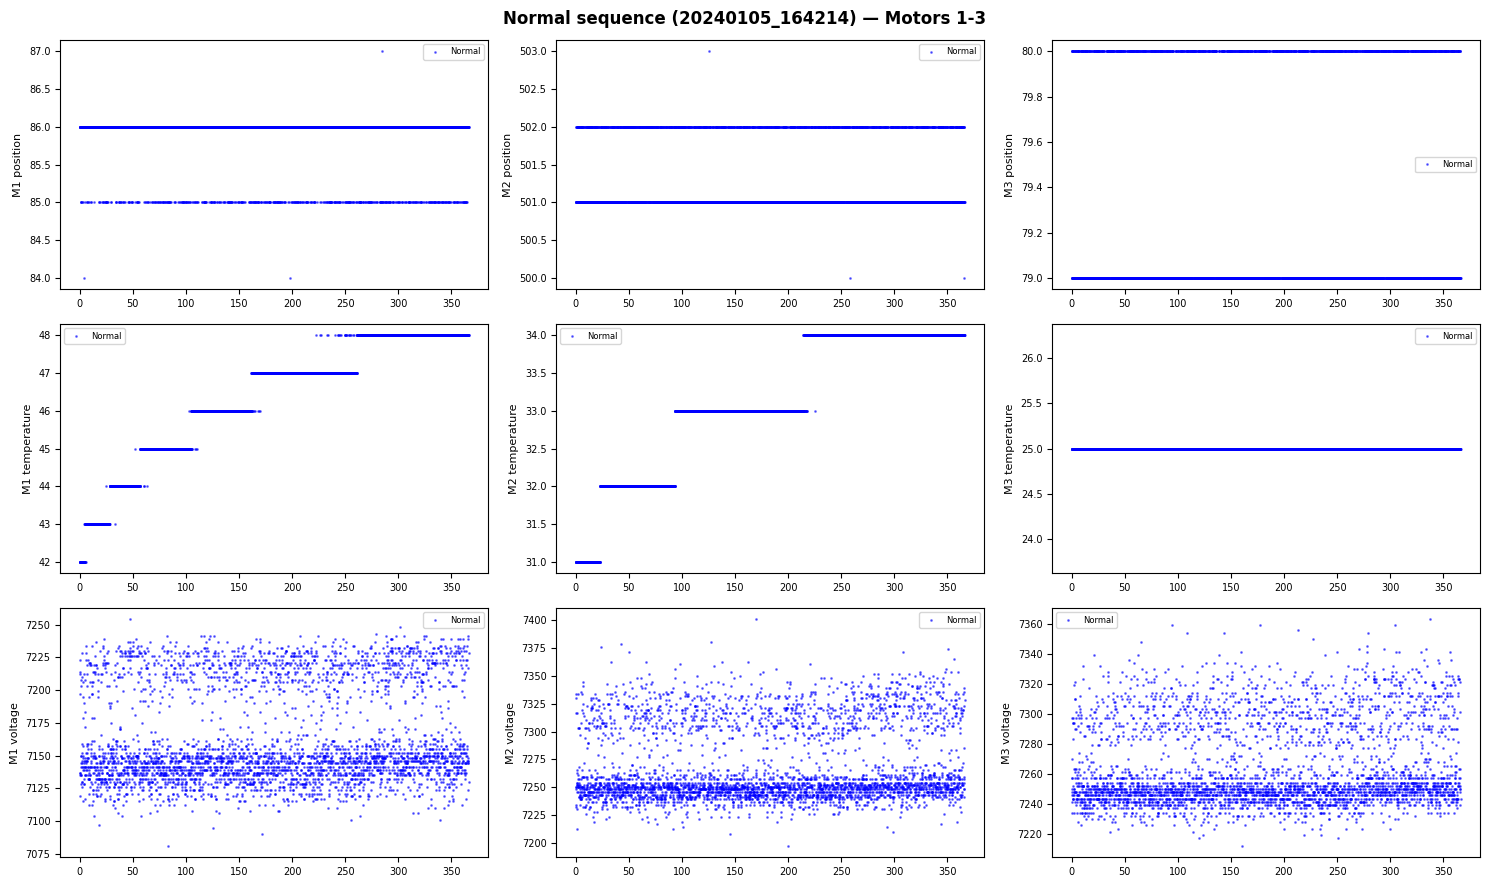
\includegraphics[width=\textwidth]{img/td4_cell006_img00.png}
  \caption{Señales crudas de la secuencia normal \texttt{20240105\_164214},
           motores 1 a 3. Azul: muestras normales (etiqueta 0).
           Observar: posición con patrón oscilatorio regular entre dos set-points,
           temperatura con tendencia suave ascendente por calentamiento progresivo,
           voltaje con fluctuaciones de alta frecuencia alrededor de $\sim$7200--7600 mV.
           Todos los puntos son azules: no hay fallos en esta secuencia.}
  \label{fig:td4_raw_normal_m13}
\end{figure}

En la figura~\ref{fig:td4_raw_normal_m13} se observa el comportamiento esperado de
los motores en operación normal:

\begin{itemize}[leftmargin=2em]
  \item \textbf{Posición:} señal cuadrada suavizada que alterna entre dos niveles
    (set-points), con transiciones relativamente rápidas. El ruido superpuesto
    es moderado y simétrico.

  \item \textbf{Temperatura:} tendencia casi lineal ascendente, típica del
    calentamiento por disipación de potencia. La señal es muy suave, con muy
    poco ruido de alta frecuencia. Esto refleja la inercia térmica del motor.

  \item \textbf{Voltaje:} la señal más ruidosa de las tres. Las fluctuaciones
    son irregulares y corresponden a variaciones en la demanda de corriente
    durante los movimientos.
\end{itemize}

\subsubsection{Secuencia normal: motores 4–6}

\begin{figure}[H]
  \centering
  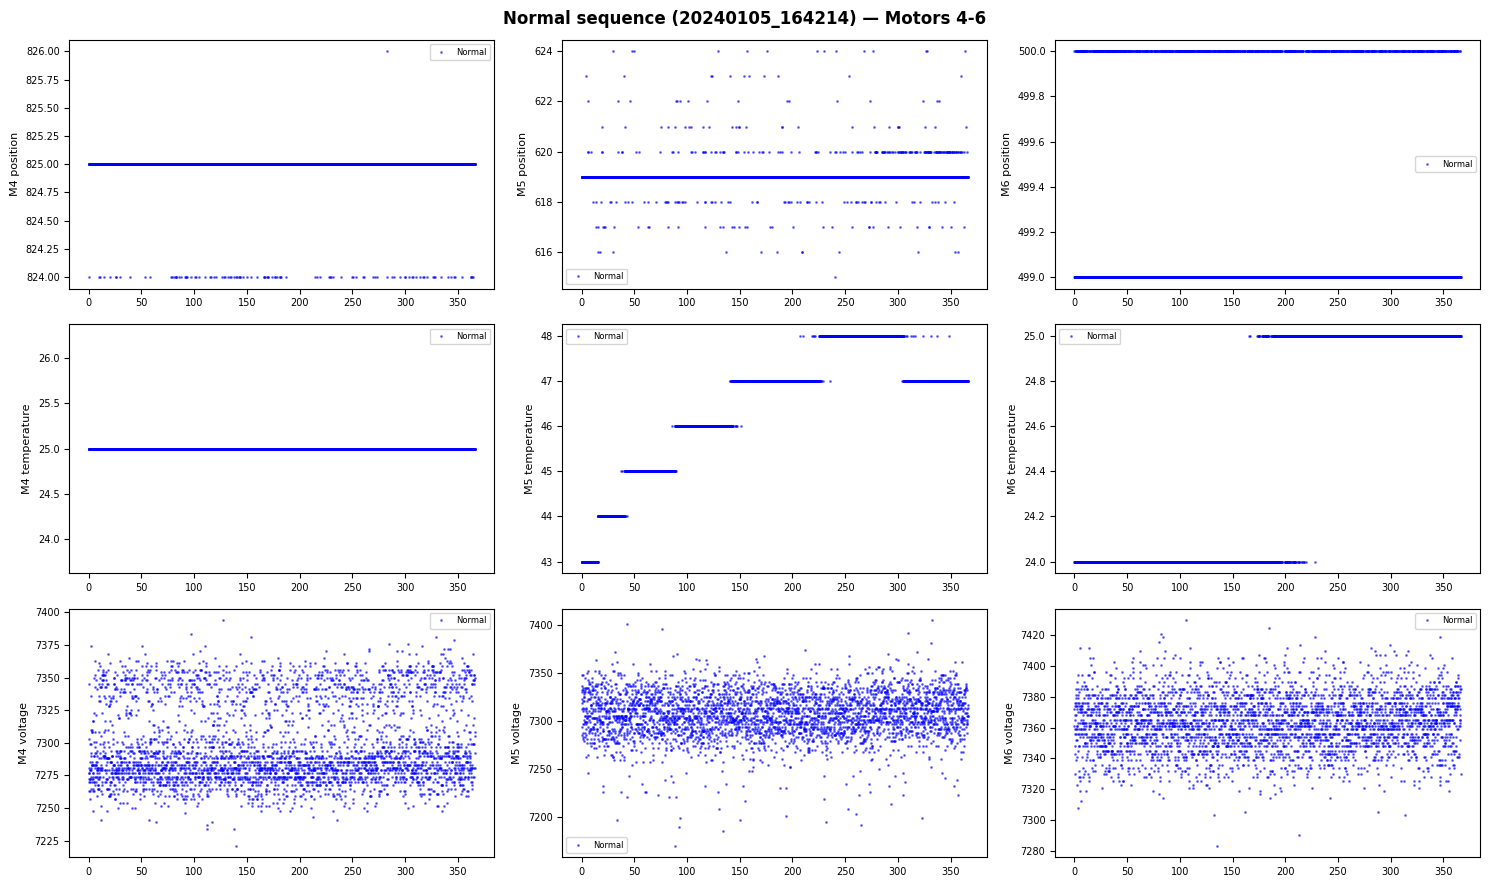
\includegraphics[width=\textwidth]{img/td4_cell006_img01.png}
  \caption{Señales crudas de la secuencia normal \texttt{20240105\_164214},
           motores 4 a 6. Azul: muestras normales. Se confirma el mismo
           patrón de los motores 1--3: posición oscilatoria, temperatura
           monotónamente creciente y voltaje ruidoso. Las escalas de
           temperatura difieren ligeramente entre motores, reflejando
           distintas condiciones de carga y flujo de calor.}
  \label{fig:td4_raw_normal_m46}
\end{figure}

La figura~\ref{fig:td4_raw_normal_m46} confirma que los motores 4--6 siguen
el mismo patrón cualitativo que los motores 1--3 en condición normal.
Se aprecia que las temperaturas de arranque de cada motor son diferentes
(distinto historial térmico antes del experimento), lo que justifica que
las temperaturas de cada motor deben tratarse como señales independientes
y no pueden mezclarse ni promediar.

\subsubsection{Secuencia con fallos: motores 1–3}

\begin{figure}[H]
  \centering
  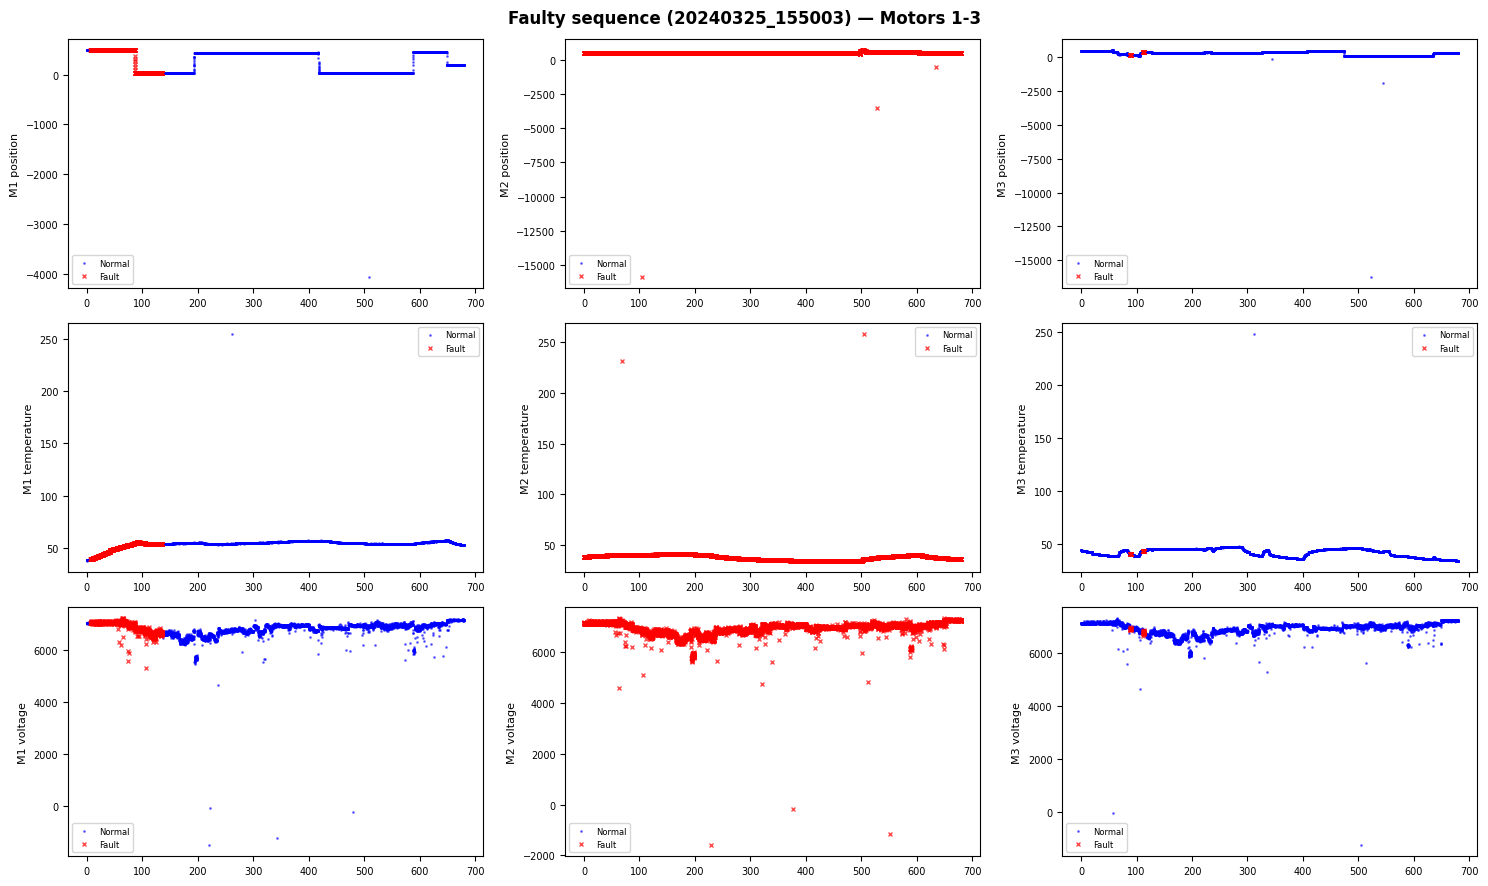
\includegraphics[width=\textwidth]{img/td4_cell006_img02.png}
  \caption{Señales crudas de la secuencia con fallos \texttt{20240325\_155003},
           motores 1 a 3. Puntos azules: muestras normales (etiqueta 0).
           Cruces rojas: muestras de fallo (etiqueta 1).
           Observar especialmente: cambios bruscos en posición y voltaje durante
           los periodos de fallo (marcados en rojo), posibles picos anómalos en
           temperatura, y que los fallos ocurren en bloques temporales continuos,
           no de forma aleatoria.}
  \label{fig:td4_raw_fault_m13}
\end{figure}

La figura~\ref{fig:td4_raw_fault_m13} muestra la secuencia más informativa del
dataset. Los puntos rojos (cruces) permiten identificar:

\begin{itemize}[leftmargin=2em]
  \item Los fallos ocurren en \textbf{bloques temporalmente continuos}, no de
    forma puntual. Esto es coherente con la naturaleza del experimento (el fallo
    se induce y mantiene durante un intervalo de tiempo).

  \item Durante los periodos de fallo, la señal de posición en algunos motores
    muestra desplazamientos sistemáticos del valor medio o cambios en la amplitud
    de oscilación.

  \item El voltaje durante el fallo puede mostrar caídas sostenidas o aumentos,
    dependiendo del tipo de fallo inducido (sobrecarga vs.\ cortocircuito parcial).

  \item Los valores anómalos de temperatura (superiores a 100 °C en algunos instantes)
    son visibles como picos aislados, confirmando los artefactos de saturación de
    sensor discutidos en las estadísticas descriptivas.
\end{itemize}

\subsubsection{Secuencia con fallos: motores 4–6}

\begin{figure}[H]
  \centering
  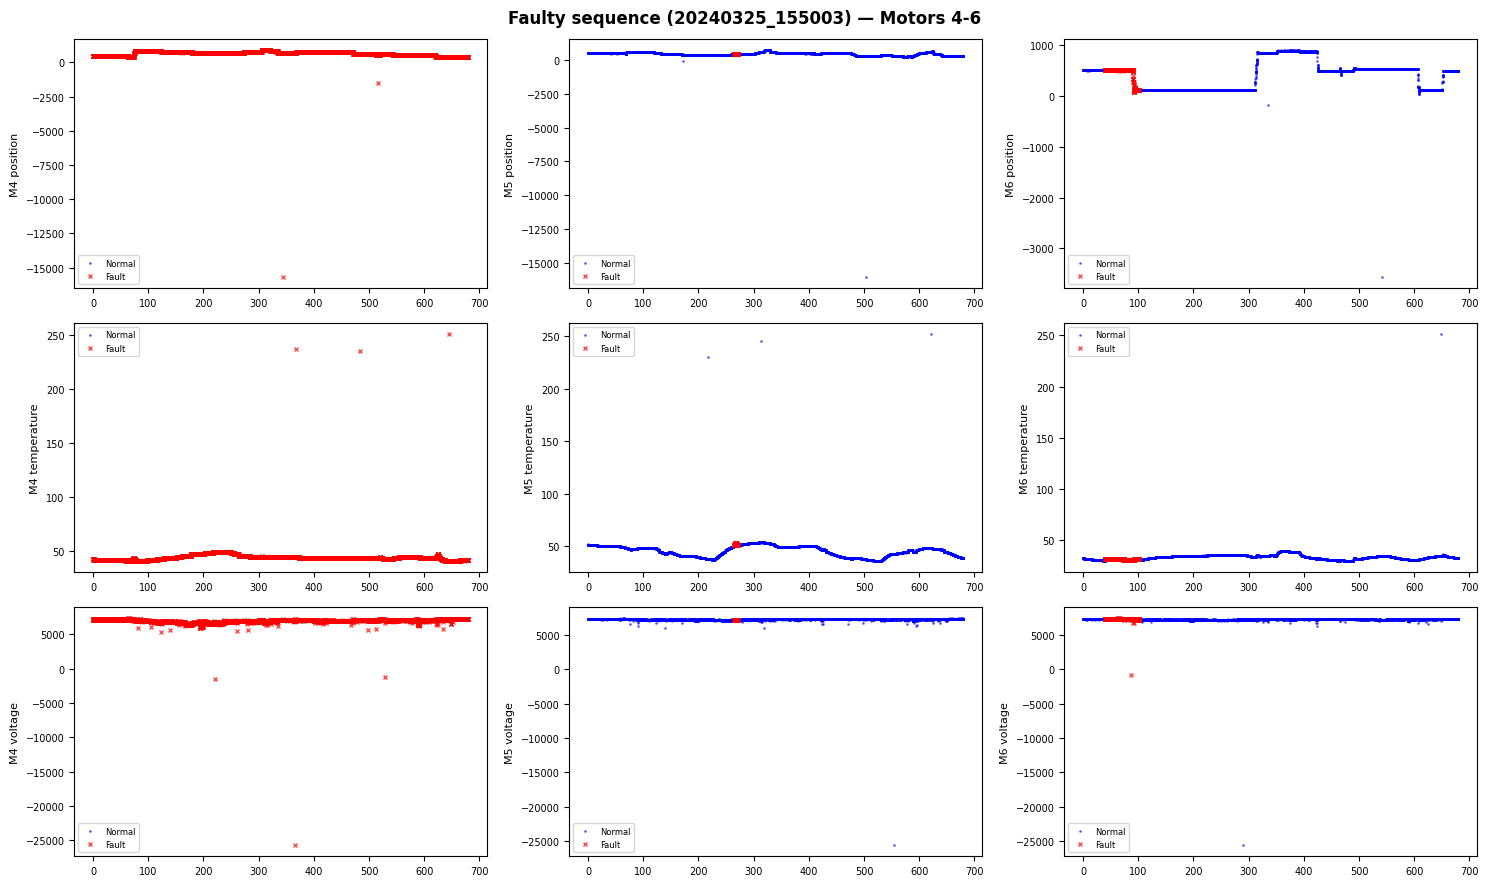
\includegraphics[width=\textwidth]{img/td4_cell006_img03.png}
  \caption{Señales crudas de la secuencia con fallos \texttt{20240325\_155003},
           motores 4 a 6. Cruces rojas: muestras de fallo. Motor 4 muestra
           los cambios más marcados: desplazamiento de posición media y caída
           de voltaje sostenida durante el fallo. Motor 5 tiene muy pocas cruces
           rojas (fallo muy raro), mientras que motor 6 muestra un comportamiento
           intermedio.}
  \label{fig:td4_raw_fault_m46}
\end{figure}

\begin{resultbox}
La inspección visual de las señales crudas confirma tres hallazgos críticos para
el diseño del pipeline:

\begin{enumerate}[leftmargin=1.5em]
  \item \textbf{Diferencias visibles entre normal y fallo existen}, especialmente
    en posición y voltaje para los motores 2 y 4. Esto valida el enfoque de
    clasificación basado en señales instantáneas.

  \item \textbf{Los picos de temperatura superiores a 100 °C son artefactos}
    (saturación ADC), no fallos reales. Deben ser eliminados en la etapa de
    limpieza por rango físico.

  \item \textbf{El voltaje es la señal más ruidosa} y requiere suavizado para
    hacer emerger la señal diagnóstica de baja frecuencia por encima del ruido
    eléctrico.
\end{enumerate}
\end{resultbox}

\subsection{Sub-tarea 3: Histogramas y Boxplots de las 18 Características}

\begin{whybox}
\textbf{Por qué histogramas y boxplots después de ver las series temporales:}
Las series temporales muestran \emph{cómo evolucionan} las señales; los histogramas
y boxplots muestran \emph{cómo se distribuyen} sus valores. Esta perspectiva
complementaria es fundamental porque:
\begin{itemize}[leftmargin=1.5em]
  \item Revela la forma de la distribución: ¿unimodal? ¿bimodal? ¿asimétrica?
    Esta información determina qué método de detección de outliers es apropiado
    (z-score vs.\ IQR vs.\ recorte por rangos físicos).
  \item Los boxplots permiten comparar visualmente los 6 motores de un mismo tipo
    de señal y detectar motores con distribuciones anómalas.
  \item La presencia de colas largas o valores extremos aislados (outliers) es
    más visible en histogramas que en series temporales densas.
\end{itemize}

\textbf{Por qué 6 motores $\times$ 3 señales = 18 subplots en una sola figura:}
Porque la comparación \emph{entre} motores para una misma señal es tan importante
como la comparación \emph{entre} señales para un mismo motor. La disposición
matricial (señal en filas, motor en columnas) facilita ambas comparaciones
simultáneamente.
\end{whybox}

\begin{lstlisting}[caption={Generación de histogramas de las 18 características}, label={lst:hist}]
import seaborn as sns

fig, axes = plt.subplots(3, 6, figsize=(18, 9))
signal_types = ['position', 'temperature', 'voltage']

for i_sig, sig in enumerate(signal_types):
    for motor in range(1, 7):
        ax = axes[i_sig, motor-1]
        col = f'data_motor_{motor}_{sig}'
        ax.hist(df[col], bins=60, edgecolor='none',
                color='steelblue', alpha=0.7)
        ax.set_title(f'M{motor}', fontsize=8)
        if motor == 1:
            ax.set_ylabel(sig[:4], fontsize=8)

plt.suptitle('Histogramas de senales por motor')
plt.tight_layout()
plt.show()
\end{lstlisting}

\begin{figure}[H]
  \centering
  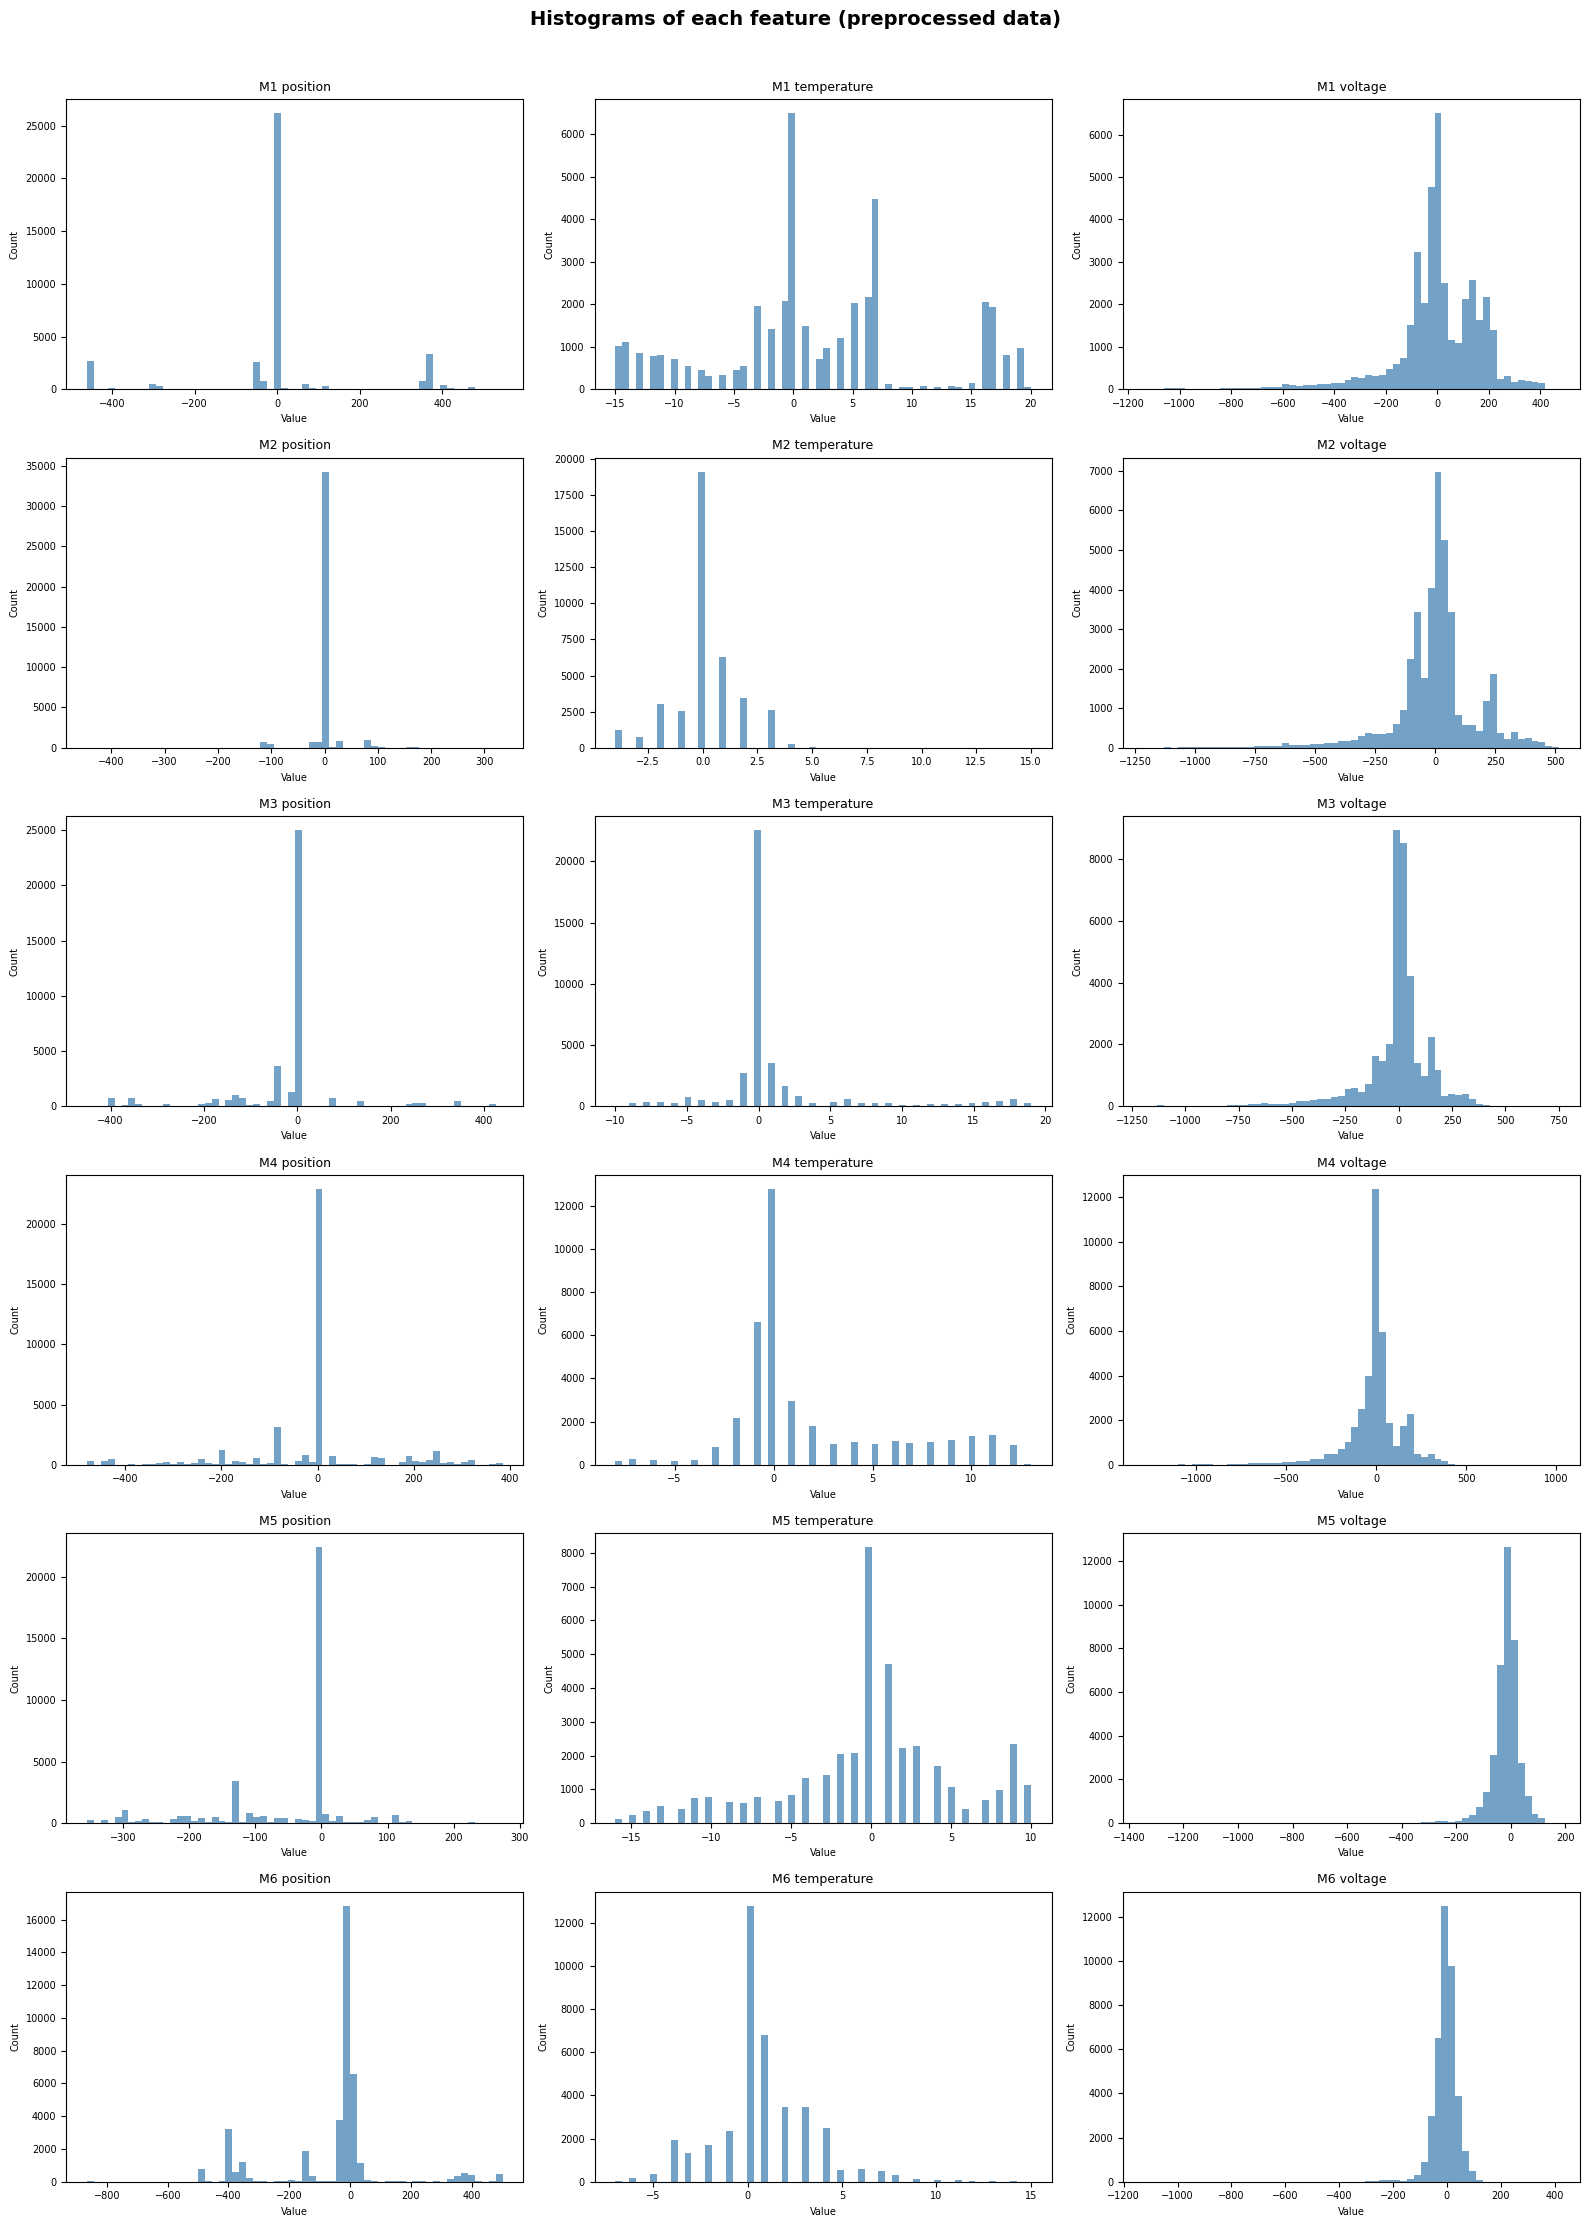
\includegraphics[width=\textwidth]{img/td4_cell011_img04.png}
  \caption{Histogramas de las 18 características del dataset (6 motores $\times$
           3 señales). Filas: posición (arriba), temperatura (centro), voltaje (abajo).
           Columnas: motores 1 a 6. Observar: distribución bimodal en posición
           (los dos set-points), colas derechas en temperatura (posibles saturaciones
           de sensor a 255 °C aparecen como barras aisladas al extremo derecho),
           y distribución aproximadamente normal en voltaje.}
  \label{fig:td4_histograms}
\end{figure}

\textbf{Hallazgos de los histogramas (figura~\ref{fig:td4_histograms}):}

\begin{itemize}[leftmargin=2em]
  \item \textbf{Posición:} distribución claramente \textbf{bimodal}. Los dos picos
    corresponden a los dos set-points entre los que el motor oscila.
    Este bimodalismo es importante para la detección de outliers: el método IQR
    (rango intercuartílico) clasificaría erróneamente como outlier hasta el 40\%
    de las muestras de posición (todas las que caen en el valle entre los dos picos),
    simplemente porque la mediana cae en una zona de baja densidad.
    El \textbf{z-score} es más robusto en este escenario porque usa la media y
    la desviación estándar globales, siendo menos sensible a la bimodalidad.

  \item \textbf{Temperatura:} distribución unimodal asimétrica, con la mayor parte de
    los valores concentrados entre 20 y 60 °C. Cola derecha pronunciada por calentamiento
    durante operación prolongada. Los outliers en 255 °C son claramente visibles como
    barras aisladas en el extremo del histograma, especialmente en los motores 1 y 4.

  \item \textbf{Voltaje:} distribución aproximadamente normal centrada alrededor de
    7200--7600 mV. Cola izquierda leve debida a caídas de tensión durante movimientos
    rápidos.
\end{itemize}

\begin{notebox}
\textbf{Por qué z-score y no IQR para detectar outliers:}
El IQR define como outlier cualquier punto fuera de $[Q1 - 1.5 \cdot \text{IQR},
Q3 + 1.5 \cdot \text{IQR}]$. Para una distribución bimodal como la posición del motor,
$Q1$ y $Q3$ pueden caer en los picos de la distribución, haciendo que el valle intermedio
(una zona \emph{completamente normal} de operación) sea marcado como outlier.
El z-score, al medir la desviación en unidades de desviación estándar global,
penaliza únicamente los extremos estadísticos genuinos.

Adicionalmente, para la temperatura existe una razón física aún más directa: sabemos
exactamente cuál es el rango físico posible [0, 100] °C. Un valor de 255 °C no es
un ``outlier estadístico'' -- es un error de sensor con causa conocida. Por eso se
usa primero recorte por rango físico y solo después z-score.
\end{notebox}

\subsubsection{Boxplots de las 18 características}

\begin{whybox}
\textbf{Por qué también boxplots si ya tenemos histogramas:}
Los boxplots complementan a los histogramas de tres formas específicas:
(1) muestran mediana, cuartiles y rango intercuartílico de forma compacta y
comparable entre motores sin necesidad de ajustar escalas de histograma;
(2) representan explícitamente los outliers como puntos individuales fuera
de los bigotes, facilitando su cuantificación visual; (3) permiten comparar
la dispersión relativa entre los 6 motores para la misma señal en un solo
vistazo. Histogramas y boxplots son complementarios: el primero muestra la
\emph{forma} de la distribución, el segundo sus \emph{estadísticos robustos}.
\end{whybox}

\begin{lstlisting}[caption={Generación de boxplots de las 18 características}, label={lst:boxplot}]
fig, axes = plt.subplots(3, 6, figsize=(18, 9))

for i_sig, sig in enumerate(signal_types):
    for motor in range(1, 7):
        ax = axes[i_sig, motor-1]
        col = f'data_motor_{motor}_{sig}'
        ax.boxplot(df[col].dropna(), whis=1.5,
                   flierprops=dict(marker='.', alpha=0.3, ms=2))
        ax.set_title(f'M{motor}', fontsize=8)
        if motor == 1:
            ax.set_ylabel(sig[:4], fontsize=8)

plt.suptitle('Boxplots de senales por motor')
plt.tight_layout()
plt.show()
\end{lstlisting}

\begin{figure}[H]
  \centering
  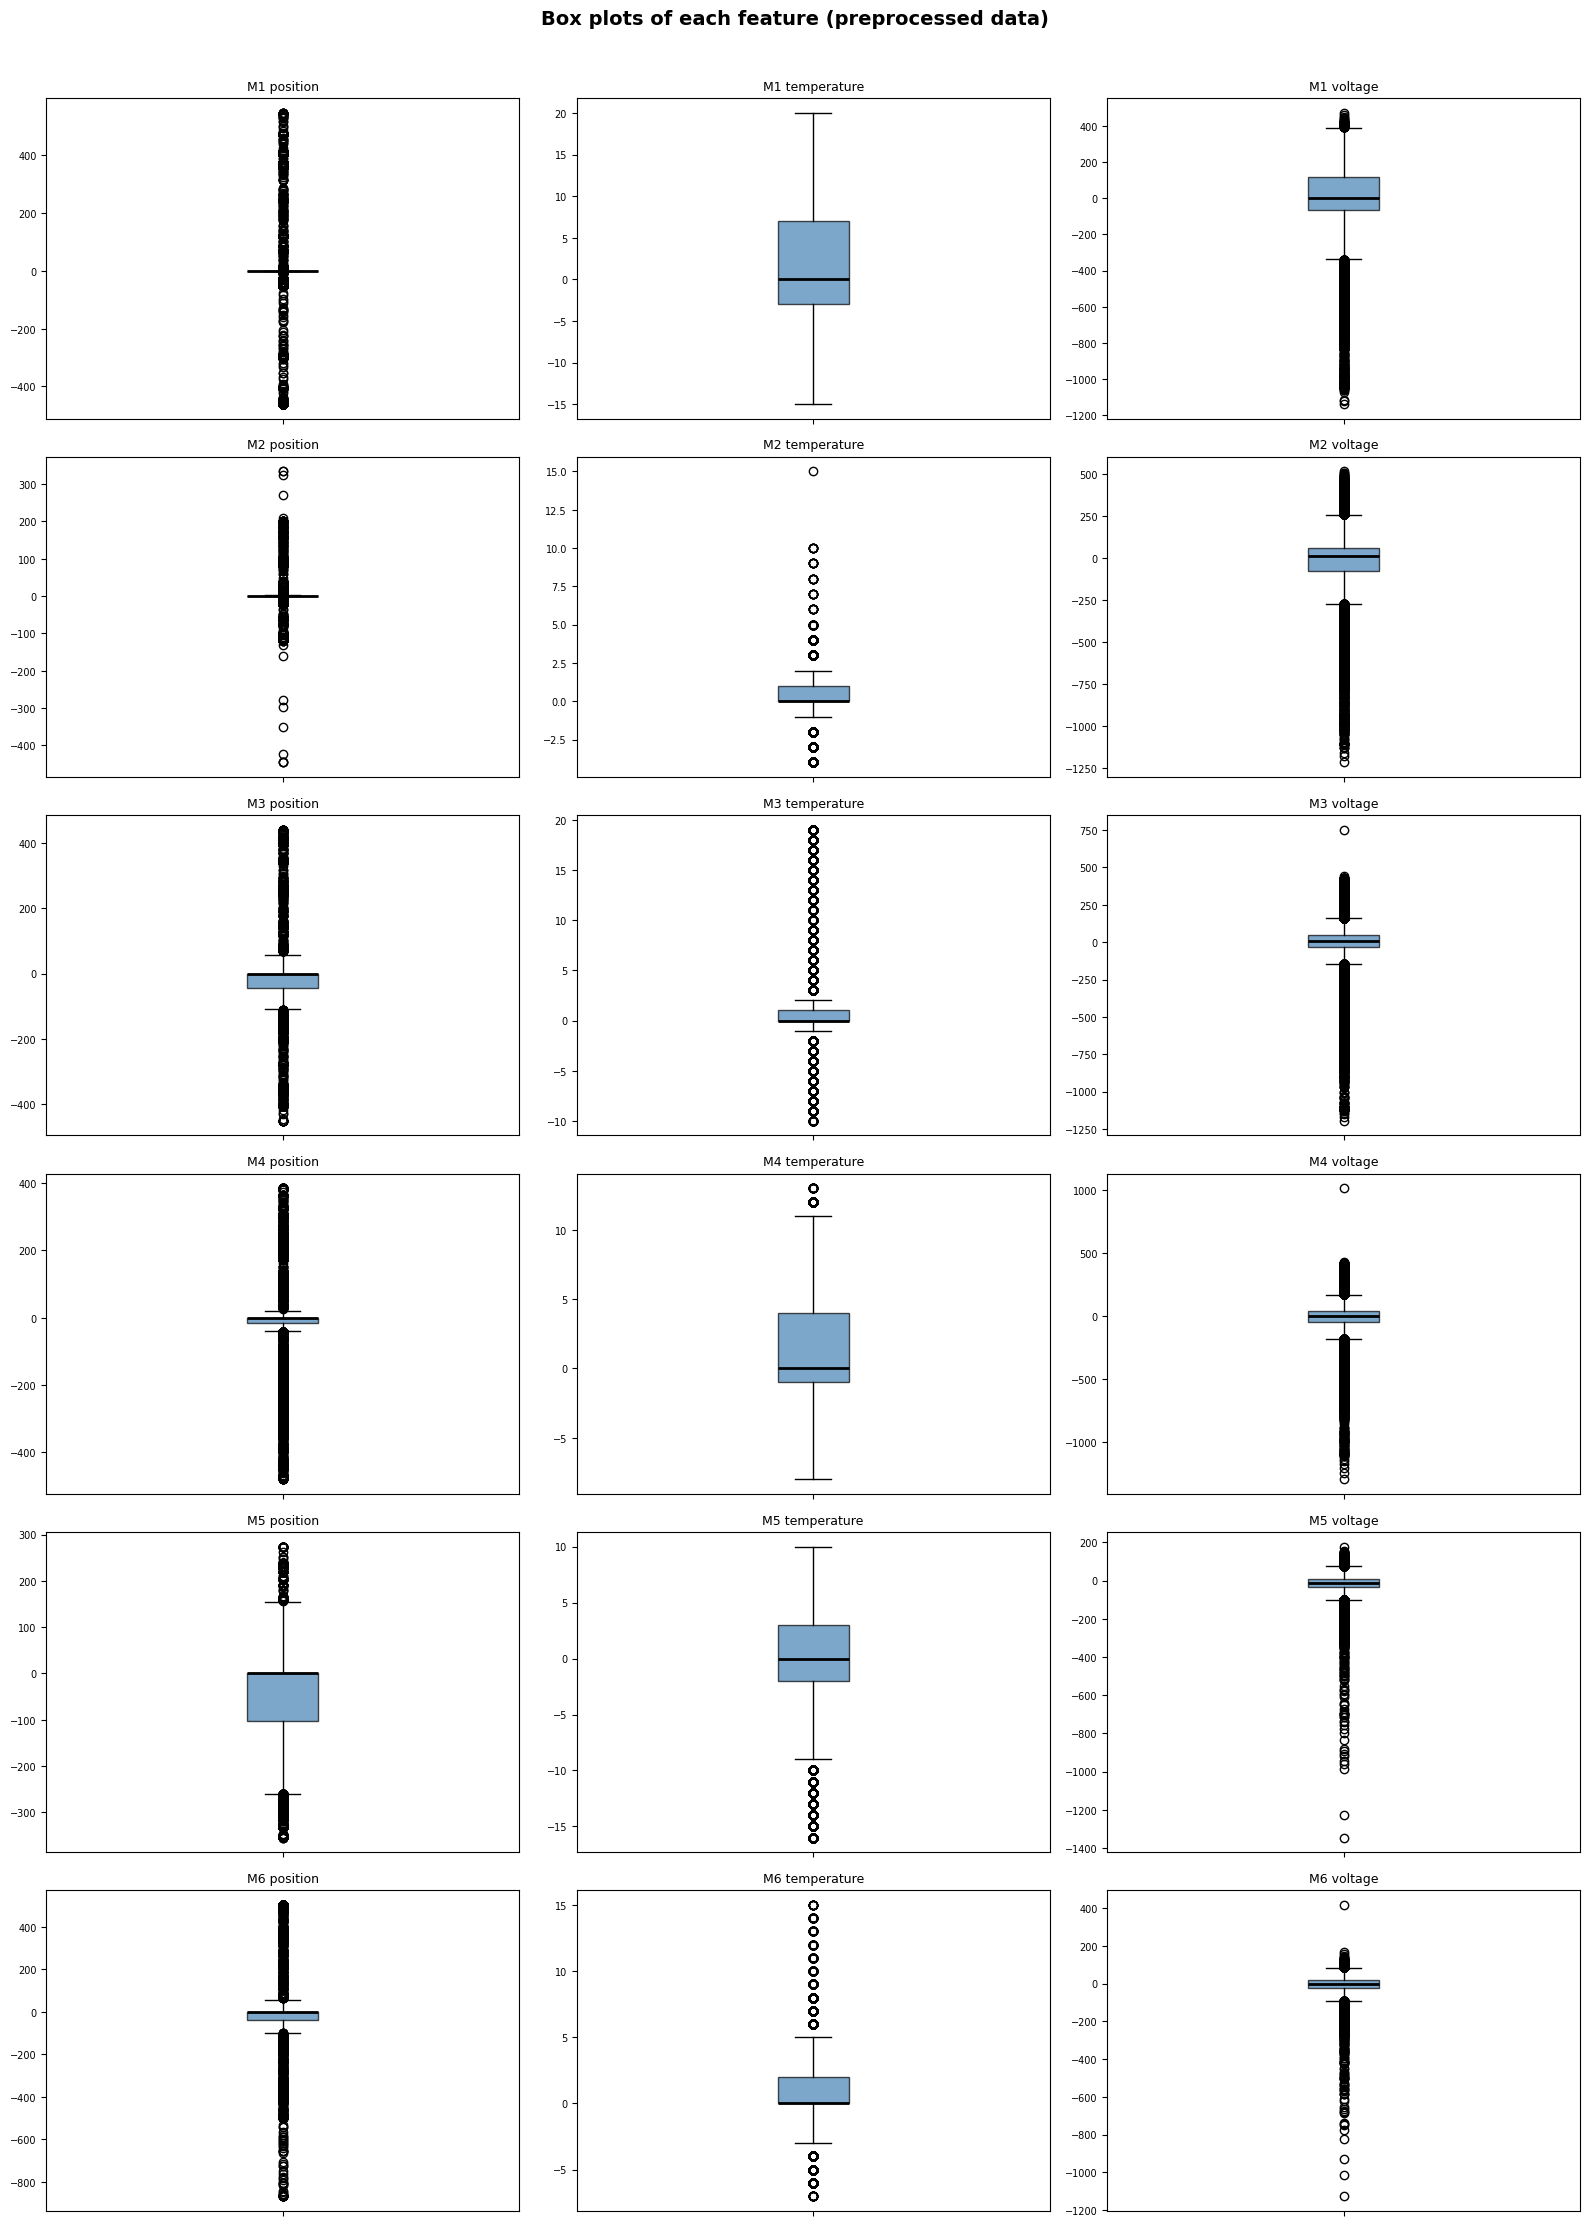
\includegraphics[width=\textwidth]{img/td4_cell012_img05.png}
  \caption{Boxplots de las 18 características (6 motores $\times$ 3 señales).
           Filas: posición (arriba), temperatura (centro), voltaje (abajo).
           Los puntos fuera de los bigotes son outliers según el criterio IQR$\times$1.5.
           Observar: gran densidad de ``outliers'' en posición (consecuencia de la
           distribución bimodal -- el IQR no es apropiado para posición), outliers
           extremos aislados en temperatura superiores a 100 °C (saturación de sensor),
           y outliers relativamente escasos en voltaje.}
  \label{fig:td4_boxplots}
\end{figure}

\textbf{Interpretación de los boxplots (figura~\ref{fig:td4_boxplots}):}

\begin{itemize}[leftmargin=2em]
  \item \textbf{Posición:} los boxplots muestran una gran cantidad de puntos fuera
    de los bigotes, pero esto es un artefacto de la distribución bimodal, no outliers
    reales. Esta es precisamente la razón por la que el IQR no debe usarse para la
    limpieza de la señal de posición.

  \item \textbf{Temperatura:} los bigotes superiores se extienden hasta $\sim 80$--100 °C
    en la mayoría de los motores, con puntos aislados en 255 °C claramente visibles.
    Estos puntos son los artefactos de saturación de sensor que deben eliminarse
    por recorte físico.

  \item \textbf{Voltaje:} distribución relativamente simétrica con pocos outliers
    verdaderos. Los rangos intercuartílicos son similares entre motores, sugiriendo
    que todos miden el mismo bus de alimentación con ruido similar.
\end{itemize}

\subsection{Sub-tarea 4: Análisis de Componentes Principales (PCA)}

\begin{whybox}
\textbf{Por qué PCA como parte de la exploración inicial:}
El PCA sirve aquí como herramienta de diagnóstico, no de reducción de
dimensionalidad para el modelo final. Aplicarlo \emph{sin} y \emph{con}
normalización tiene dos objetivos distintos:

\begin{enumerate}[leftmargin=1.5em]
  \item \textbf{Sin normalización:} demostrar empíricamente el efecto de la
    diferencia de escalas entre señales. Si el PCA sin normalizar está dominado
    por una sola señal (voltaje), queda evidenciada la necesidad de normalizar.

  \item \textbf{Con normalización:} revelar la verdadera estructura dimensional
    de los datos. ¿Cuántas dimensiones independientes tiene la información contenida
    en las 18 señales? ¿Existe alguna separabilidad visual en el espacio 2D entre
    normal y fallo?
\end{enumerate}

\textbf{Por qué no usar PCA directamente para selección de características:}
El PCA crea combinaciones lineales de todas las variables, perdiendo la
interpretabilidad física de las señales originales. Para un sistema industrial
donde ``la temperatura del motor 4 es alta'' tiene significado para el operario,
preferimos conservar las variables originales y aplicar selección de características
basada en relevancia y redundancia.
\end{whybox}

\begin{lstlisting}[caption={PCA sin y con normalización}, label={lst:pca}]
from sklearn.decomposition import PCA
from sklearn.preprocessing import StandardScaler, MinMaxScaler
import numpy as np

# Seleccionar solo las 18 caracteristicas de senales
feature_cols = [c for c in df.columns
                if any(s in c for s in
                       ['position','temperature','voltage'])]
X = df[feature_cols].dropna().values
y = df.loc[df[feature_cols].notna().all(axis=1),
           'data_motor_1_label'].values   # etiqueta ilustrativa

# ---- Sin normalizacion ----
pca_raw = PCA(n_components=2)
X_pca_raw = pca_raw.fit_transform(X)
var_raw = pca_raw.explained_variance_ratio_
print("Varianza explicada (sin norm):", var_raw.cumsum()[:2])
# [0.699, 0.712]  -- PC1~70%, acumulado 2 comps~71%

# ---- Con StandardScaler ----
Xs = StandardScaler().fit_transform(X)
pca_std = PCA(n_components=18)
pca_std.fit(Xs)
cumvar = np.cumsum(pca_std.explained_variance_ratio_)
print("Var acumulada (std):", cumvar[:8])
# [0.28, 0.46, 0.57, 0.65, 0.72, 0.78, 0.83, 0.87]

n85 = np.argmax(cumvar >= 0.85) + 1
print(f"Componentes para 85% varianza: {n85}")  # 8
\end{lstlisting}

\subsubsection{PCA sin normalización: dominio del voltaje}

\begin{figure}[H]
  \centering
  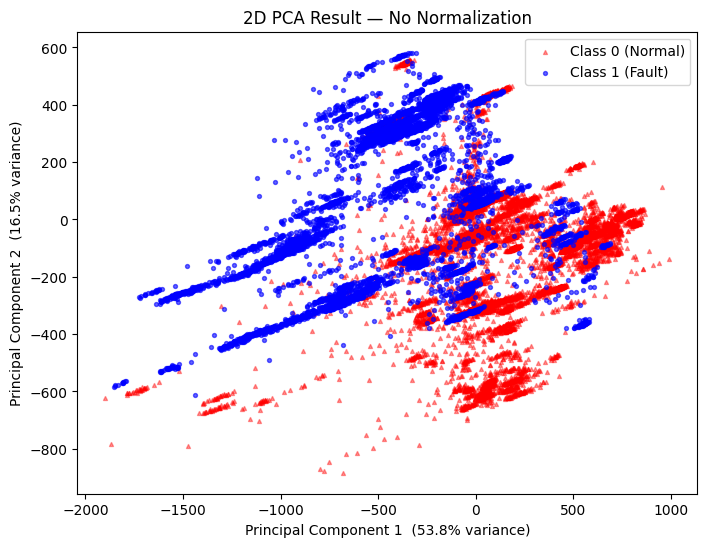
\includegraphics[width=0.72\textwidth]{img/td4_cell014_img06.png}
  \caption{PCA 2D aplicado sobre los datos \textbf{sin normalización}.
           Rojo: clase normal (etiqueta 0). Azul: clase fallo (etiqueta 1).
           La PC1 (eje horizontal) captura el $\approx 70\%$ de la varianza y está
           alineada casi exclusivamente con la dirección de variación del voltaje
           (escala $\sim$3000 mV de rango). Observar que la separación entre
           normal (rojo) y fallo (azul) es pobre en este espacio: la dominancia
           del voltaje oculta la información diagnóstica de otras señales.}
  \label{fig:td4_pca_raw}
\end{figure}

Cuando se aplica PCA directamente sobre los datos brutos (figura~\ref{fig:td4_pca_raw}),
el voltaje (escala $\sim 3000$ mV de rango) domina completamente la varianza.
La PC1 captura aproximadamente el \textbf{70\% de la varianza total} y está alineada casi
exclusivamente con la dirección de variación del voltaje. Los dos primeros
componentes explican en conjunto $\approx 71\%$ de la varianza.
\textbf{Esta alta proporción es engañosa}: no refleja la estructura real de los
datos sino simplemente la diferencia de escala entre señales.

La separabilidad visual entre clases en este espacio 2D es limitada porque la PC1
(que domina la representación) está orientada principalmente por el voltaje, que
tiene cierto poder discriminativo pero no el mejor. La información de temperatura
(buen discriminador para motores 1 y 6) queda comprimida en componentes de menor
varianza que no aparecen en este gráfico 2D.

\subsubsection{PCA con normalización: revelando la estructura real}

\begin{figure}[H]
  \centering
  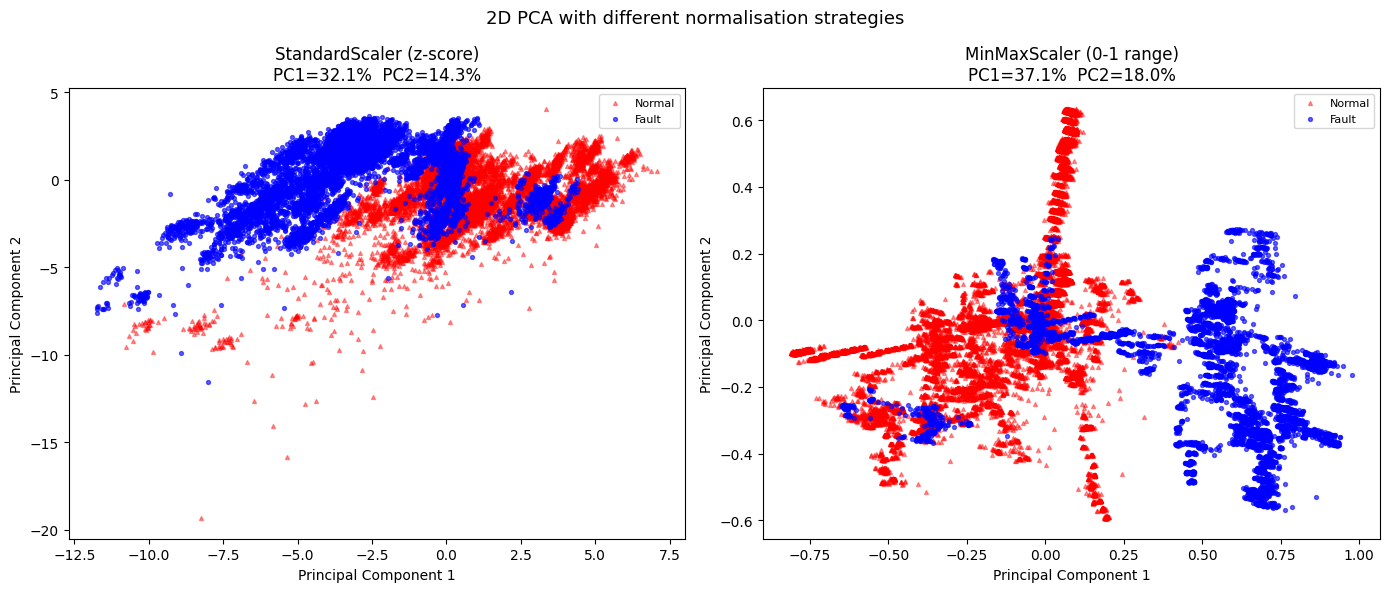
\includegraphics[width=\textwidth]{img/td4_cell016_img07.png}
  \caption{PCA 2D comparando \textbf{StandardScaler} (izquierda) y \textbf{MinMaxScaler}
           (derecha) como estrategias de normalización previas al PCA.
           Rojo: clase normal. Azul: clase fallo.
           Con StandardScaler, los dos primeros componentes explican $\approx 46\%$
           de la varianza, con mejor separación entre clases que sin normalización.
           Con MinMaxScaler se obtiene una distribución de puntos similar aunque
           con mayor sensibilidad a los outliers de los extremos.
           En ambos casos el solapamiento parcial entre clases confirma que se
           necesitan clasificadores no lineales.}
  \label{fig:td4_pca_scaled}
\end{figure}

\begin{whybox}
\textbf{Por qué StandardScaler y no MinMaxScaler:}
El gráfico de la figura~\ref{fig:td4_pca_scaled} muestra visualmente la diferencia.
Cuantitativamente:

\begin{itemize}[leftmargin=1.5em]
  \item \textbf{StandardScaler} ($z = (x-\mu)/\sigma$): transforma cada señal para
    tener media 0 y varianza 1. Un outlier extremo (ej. temperatura de 255 °C)
    se convierte en un valor grande pero finito (ej. $z \approx +15$), que queda
    fuera de la nube de datos pero no deforma la distribución del resto de puntos.

  \item \textbf{MinMaxScaler} ($z = (x-x_{min})/(x_{max}-x_{min})$): si hay un
    outlier a 255 °C, $x_{max} = 255$ y el resto de valores (todos entre 0--100 °C)
    quedan comprimidos en el rango [0, 0.39], perdiendo resolución y distorsionando
    la representación de la distribución normal.
\end{itemize}

Dado que los datos tienen outliers conocidos antes de la limpieza, el StandardScaler
es más robusto. Tras la limpieza (outliers eliminados), ambos métodos serían
más comparables, pero por coherencia del pipeline se mantiene StandardScaler.
\end{whybox}

Al normalizar previamente (media 0, varianza 1 por característica), la varianza
queda repartida de forma más equitativa entre las 18 señales.
Ahora los dos primeros componentes explican solo \textbf{$\approx 46\%$} de la
varianza, lo que indica que los datos son genuinamente \textbf{multidimensionales}:
ningún par de direcciones ortogonales captura la mayor parte de la información.

\begin{table}[H]
\centering
\caption{Varianza explicada acumulada con StandardScaler}
\begin{tabular}{@{}cc@{}}
\toprule
\textbf{Número de componentes} & \textbf{Varianza explicada acumulada (\%)}\\
\midrule
1  & 28\%\\
2  & 46\%\\
3  & 57\%\\
4  & 65\%\\
5  & 72\%\\
6  & 78\%\\
7  & 83\%\\
8  & 87\%\\
\bottomrule
\end{tabular}
\end{table}

\begin{resultbox}
Se necesitan \textbf{8 componentes principales} para capturar el 85\% de la varianza
cuando los datos están correctamente normalizados. Esto sugiere que las 18 señales
aportan información genuinamente independiente, aunque con cierta redundancia
(especialmente entre los voltajes de distintos motores, que están muy correlacionados).

En el gráfico 2D del PCA con normalización (figura~\ref{fig:td4_pca_scaled}),
los puntos de clase normal y fallo muestran un \textbf{solapamiento parcial}:
aunque existen regiones con predominio de una clase, las dos nubes no están
limpiamente separadas. Esto confirma que la detección de fallos requiere
clasificadores no lineales y que las señales brutas por sí solas no son
suficientes sin ingeniería de características.
\end{resultbox}

% ============================================================
\section{Task 2: Limpieza y Preprocesamiento}

\subsection{Sub-tarea 1: Normalización}

\subsubsection{Motivación y elección de la estrategia}

\begin{whybox}
\textbf{Por qué normalizar es necesario en este dataset:}
Como se evidenció en el PCA, las tres señales operan en escalas completamente distintas:
posición [0, 1000], temperatura [0, 100], voltaje [6000, 9000]. La diferencia de
magnitudes es de varios órdenes: el voltaje tiene valores medios $\sim$150 veces
mayores que la temperatura.

Si no se normaliza:
\begin{enumerate}[leftmargin=1.5em]
  \item \textbf{Distancias euclidianas} (k-NN, k-Means, SVM RBF): la distancia
    estará dominada por diferencias en voltaje (rango 3000) mientras que la
    temperatura (rango 100) tendrá peso $\sim 30\times$ menor. El modelo ignorará
    efectivamente temperatura y posición.
  \item \textbf{Gradientes} (regresión logística, redes neuronales): los pesos
    asociados al voltaje recibirán gradientes $\sim 30\times$ mayores, haciendo
    el entrenamiento inestable y convergencia lenta.
  \item \textbf{PCA}: como se demostró, la primera componente estará alineada con
    voltaje independientemente de su relevancia diagnóstica real.
\end{enumerate}

\textbf{Los árboles de decisión (Random Forest, XGBoost) son inmunes a la escala}
porque sus divisiones comparan valores de la misma columna entre sí. Sin embargo,
normalizar no perjudica a los árboles y facilita la comparación de importancias de
variables entre señales de distintas escalas.
\end{whybox}

\subsubsection{División Train/Test a Nivel de Secuencia}

\begin{notebox}
La división train/test debe realizarse \textbf{a nivel de secuencia}, no de fila.
Si se dividiese aleatoriamente por filas, muestras temporalmente adyacentes de la
misma secuencia aparecerían en train y en test simultáneamente, provocando
\textbf{data leakage temporal}: el modelo vería (indirectamente) el futuro del test
durante el entrenamiento.

En series temporales industriales, la unidad mínima de independencia es la secuencia
de test completa, no la muestra individual. Dos muestras consecutivas de la misma
secuencia están fuertemente correlacionadas (especialmente la temperatura, que cambia
despacio). Si se ponen en conjuntos distintos, el test ``conoce'' el contexto del
train adyacente.
\end{notebox}

\begin{lstlisting}[caption={Split train/test a nivel de secuencia}, label={lst:split}]
from sklearn.model_selection import train_test_split

# Obtener lista de secuencias y dividir 80/20
sequences = df['test_condition'].unique()
train_seqs, test_seqs = train_test_split(
    sequences, test_size=0.2, random_state=42
)

# Crear subsets por mascara
df_train = df[df['test_condition'].isin(train_seqs)].copy()
df_test  = df[df['test_condition'].isin(test_seqs)].copy()

print(f"Train: {len(df_train):,} filas ({len(train_seqs)} secuencias)")
# Train: 35,217 filas (18 secuencias)
print(f"Test:  {len(df_test):,} filas ({len(test_seqs)} secuencias)")
# Test:  4,092 filas  (5 secuencias)
\end{lstlisting}

\subsubsection{Aplicación del StandardScaler}

\begin{lstlisting}[caption={Ajuste y transformación con StandardScaler}, label={lst:scaler}]
from sklearn.preprocessing import StandardScaler

feature_cols = [c for c in df.columns
                if any(s in c for s in
                       ['position','temperature','voltage'])]

scaler = StandardScaler()

# Ajustar SOLO en datos de entrenamiento
X_train = scaler.fit_transform(df_train[feature_cols])

# Aplicar los MISMOS parametros al test (evita leakage)
X_test = scaler.transform(df_test[feature_cols])

# Verificar resultado
print("Media train post-norm:",  X_train.mean(axis=0).round(4))
# ~[0. 0. 0. 0. 0. 0. ...]   (cercana a 0)
print("Std train post-norm:",    X_train.std(axis=0).round(4))
# ~[1. 1. 1. 1. 1. 1. ...]   (cercana a 1)
\end{lstlisting}

\textbf{Por qué no usar \texttt{fit\_transform} también en test:}
Si se hiciera \texttt{scaler\_test.fit\_transform(X\_test)}, se calcularían
nuevos parámetros de media y varianza basados en el conjunto de test, haciendo
que train y test estén normalizados con parámetros \emph{diferentes}. El modelo,
entrenado con la escala del train, recibiría datos de test en una escala distinta,
degradando las predicciones.

\subsubsection{Comparación: StandardScaler vs.\ MinMaxScaler vs.\ RobustScaler}

\begin{table}[H]
\centering
\caption{Comparación de estrategias de normalización}
\begin{tabular}{@{}lp{4.8cm}p{5.5cm}@{}}
\toprule
\textbf{Método} & \textbf{Fórmula} & \textbf{Ventajas / Inconvenientes}\\
\midrule
StandardScaler
  & $z = \dfrac{x - \mu}{\sigma}$
  & Robusto frente a outliers moderados. Salida no acotada:
    outliers extremos siguen siendo grandes pero finitos.
    \textbf{Elección de este pipeline.}\\[0.6em]
MinMaxScaler
  & $z = \dfrac{x - x_{\min}}{x_{\max} - x_{\min}}$
  & Escala al rango [0,1]. Muy sensible a outliers: un único valor a
    255 °C comprime toda la distribución. \textbf{Descartado.}\\[0.6em]
RobustScaler
  & $z = \dfrac{x - Q_{50}}{Q_{75} - Q_{25}}$
  & Usa mediana y IQR, muy robusto a outliers extremos.
    Apropiado si hay muchos outliers antes de limpiar.
    \textbf{Alternativa válida pero innecesaria tras limpieza.}\\
\bottomrule
\end{tabular}
\end{table}

Para este dataset se elige \textbf{StandardScaler} porque la eliminación de outliers
se aplica antes de la normalización en el pipeline final, mitigando la sensibilidad
a valores extremos. El MinMaxScaler fue explícitamente descartado tras observar
su comportamiento en la figura~\ref{fig:td4_pca_scaled}.

\subsection{Sub-tarea 2: Eliminación de Outliers}

\subsubsection{Estrategia en Dos Etapas: Justificación del Enfoque}

\begin{whybox}
\textbf{Por qué dos etapas y no una sola:}
Los outliers en este dataset provienen de \textbf{dos fuentes distintas} que requieren
tratamiento diferente:

\begin{enumerate}[leftmargin=1.5em]
  \item \textbf{Errores de sensor con causa conocida} (saturación ADC a 255 °C):
    estos no son estadísticamente extremos \emph{dentro del dataset} si hay suficientes
    muestras saturadas; son físicamente imposibles. El único criterio válido es el
    conocimiento del dominio: rango físico del sensor.

  \item \textbf{Ruido estadístico extremo sin causa física conocida}: transitorios
    eléctricos, interferencias momentáneas, errores de cuantización. Estos sí deben
    detectarse mediante criterio estadístico (z-score), calculado \emph{dentro de cada
    secuencia} para no mezclar las estadísticas de operaciones diferentes.
\end{enumerate}

\textbf{Por qué calcular z-score por secuencia y no globalmente:}
Cada secuencia tiene condiciones diferentes de temperatura de arranque, carga y
duración. Si se calcula el z-score globalmente, una secuencia con temperatura media
de 60 °C podría marcar como outlier valores normales de otra secuencia con
temperatura media de 80 °C. El z-score por secuencia normaliza respecto a las
condiciones de ese experimento específico.

\textbf{Alternativa descartada:} isolation forest o DBSCAN para detección de
outliers multivariante. Si bien más sofisticados, son más lentos y menos
interpretables. Para este problema donde los rangos físicos son conocidos, el
enfoque en dos etapas es más apropiado y explicable a un operario industrial.
\end{whybox}

\textbf{Etapa 1 -- Recorte por rango físico:}
Se anulan los valores que violan los límites conocidos del sistema físico.
Un valor de temperatura de 255 °C no puede ser real en un motor servo-robótico de
uso industrial; es un artefacto de saturación del sensor (el registro de 8 bits
saturado al valor 0xFF = 255).

\begin{lstlisting}[caption={Etapa 1: Recorte por rango físico con forward-fill}, label={lst:clip}]
import numpy as np

# Definir rangos fisicos validos
physical_limits = {
    'position':    (0,    1000),
    'temperature': (0,    100),
    'voltage':     (6000, 9000),
}

df_clean = df.copy()

for sig, (lo, hi) in physical_limits.items():
    cols = [c for c in df.columns if sig in c and 'label' not in c]
    for col in cols:
        mask_out = (df_clean[col] < lo) | (df_clean[col] > hi)
        df_clean.loc[mask_out, col] = np.nan

# Forward-fill por secuencia (usar valor anterior valido)
df_clean = df_clean.groupby('test_condition', group_keys=False).apply(
    lambda g: g.fillna(method='ffill')
)
\end{lstlisting}

\textbf{Etapa 2 -- Z-score por secuencia:}
Dentro de cada secuencia, se identifica y elimina cualquier muestra cuyo z-score
supere el umbral $|z| > 3$ (equivalente a estar a más de 3 desviaciones estándar
de la media, lo que ocurre con probabilidad $< 0.27\%$ en una distribución normal).
El z-score se calcula por secuencia para no mezclar estadísticas de operaciones
distintas.

\begin{lstlisting}[caption={Etapa 2: Z-score por secuencia}, label={lst:zscore}]
from scipy import stats

ZSCORE_THRESHOLD = 3.0

def remove_outliers_zscore(group, cols, threshold=3.0):
    """Anula valores con |z| > threshold dentro de una secuencia."""
    g = group.copy()
    for col in cols:
        z = np.abs(stats.zscore(g[col].dropna()))
        idx_out = g[col].dropna().index[z > threshold]
        g.loc[idx_out, col] = np.nan
    return g.fillna(method='ffill')

feature_cols_only = [c for c in df_clean.columns
                     if any(s in c for s in
                            ['position','temperature','voltage'])]

df_clean = df_clean.groupby(
    'test_condition', group_keys=False
).apply(remove_outliers_zscore, cols=feature_cols_only)
\end{lstlisting}

\subsubsection{Resumen de Outliers Eliminados}

La siguiente tabla muestra el conteo de outliers eliminados por motor y tipo de señal
en el dataset completo de 39.309 muestras:

\begin{table}[H]
\centering
\caption{Outliers eliminados por motor y señal (ambas etapas combinadas)}
\begin{tabular}{@{}lccccc@{}}
\toprule
\textbf{Motor} & \textbf{Posición} & \textbf{Temperatura} & \textbf{Voltaje}
               & \textbf{Total motor} & \textbf{\% de filas}\\
\midrule
Motor 1 & 400 & 531 & 449 & 1.380 & 3.51\%\\
Motor 2 & 241 & 342 & 547 & 1.130 & 2.88\%\\
Motor 3 & 279 & 166 & 529 &   974 & 2.48\%\\
Motor 4 & 651 & 113 & 463 & 1.227 & 3.12\%\\
Motor 5 & 385 & 346 & 546 & 1.277 & 3.25\%\\
Motor 6 & 385 & 111 & 356 &   852 & 2.17\%\\
\midrule
\textbf{Total} & \textbf{2.341} & \textbf{1.609} & \textbf{2.890}
               & \textbf{6.840} & \textbf{0.967\%}\\
\bottomrule
\end{tabular}
\end{table}

\begin{resultbox}
En total se eliminaron \textbf{6.840 outliers}, equivalentes al \textbf{0.967\%}
de todos los valores de características ($39.309 \times 18 = 707.562$ valores en total).
Este porcentaje es moderado y coherente con la presencia de ruido de sensor moderado
y algunos artefactos de saturación.

El motor 4 tiene la mayor tasa de outliers en posición (651 muestras), lo cual es
consistente con el hecho de que también tiene la mayor tasa de fallo (17\%) y el
mayor poder discriminativo en la señal de posición.

La temperatura tiene el mayor número de outliers físicos (saturaciones a 255 °C),
mientras que el voltaje domina los outliers estadísticos (z-score), reflejando sus
respectivos mecanismos de ruido.
\end{resultbox}

\subsubsection{Forward-Fill: Justificación}

Tras anular un valor outlier, es necesario imputar un valor razonable.
Se usa \textbf{forward-fill} (rellenar con el último valor válido anterior) porque:

\begin{enumerate}[leftmargin=2em]
  \item Las señales físicas son continuas: el valor más probable en el instante $t$
    tras una muestra anómala es el valor en $t - 0.1$ s.
  \item Es \textbf{causal}: no usa información futura, por lo que no introduce
    data leakage temporal.
  \item Preserva las tendencias temporales (p.ej., el incremento gradual de temperatura).
\end{enumerate}

Si el primer valor de una secuencia es un outlier (y por tanto el forward-fill no
tiene valor previo disponible), se complementa con \textbf{backward-fill} para
ese caso específico.

\subsection{Sub-tarea 3: Suavizado Temporal con Rolling Mean}

\subsubsection{Motivación y diseño del suavizado}

\begin{whybox}
\textbf{Por qué suavizar después de eliminar outliers y no antes:}
El orden importa. Si se suaviza \emph{antes} de eliminar outliers, un pico de
temperatura a 255 °C se ``difunde'' a los 4 puntos adyacentes (ventana de 5 muestras),
contaminando valores que originalmente eran correctos. Al eliminar primero los outliers
y rellenar con forward-fill, el suavizado posterior opera sobre datos ya limpios,
obteniendo el beneficio del filtrado de ruido sin el efecto de contaminación de
artefactos.

\textbf{Por qué rolling mean y no filtro Butterworth o Kalman:}
\begin{itemize}[leftmargin=1.5em]
  \item \textbf{Rolling mean (media móvil)}: simple, interpretable, computacionalmente
    trivial, sin parámetros de frecuencia de corte a ajustar. Suficiente para el
    nivel de ruido presente en las señales.
  \item \textbf{Filtro Butterworth}: mayor control sobre la frecuencia de corte,
    pero requiere estimación de la frecuencia de corte óptima y aplica filtrado
    bidireccional en scikit-signal (no causal) si no se implementa cuidadosamente.
  \item \textbf{Filtro de Kalman}: óptimo para ruido gaussiano con modelo dinámico
    conocido. Requiere modelar la dinámica del sistema (posición, temperatura, voltaje),
    lo cual está fuera del alcance de este TD.
\end{itemize}

Para el nivel de ruido presente y la frecuencia de muestreo de 10 Hz, la media
móvil de ventana 5 (0.5 s) es suficiente y apropiada.
\end{whybox}

\begin{lstlisting}[caption={Suavizado con media móvil causal por secuencia}, label={lst:smooth}]
WINDOW_SIZE = 5    # 5 muestras = 0.5 s a 10 Hz

def smooth_sequence(group, cols, window=5):
    """Media movil causal por columna dentro de una secuencia."""
    g = group.copy()
    for col in cols:
        g[col] = g[col].rolling(
            window=window,
            center=False,      # CAUSAL: solo usa pasado
            min_periods=1      # no descarta primeras muestras
        ).mean()
    return g

df_smooth = df_clean.groupby(
    'test_condition', group_keys=False
).apply(smooth_sequence, cols=feature_cols_only)

print("Suavizado aplicado. Shape:", df_smooth.shape)
# (39309, 26)  -- mismas dimensiones, senales mas suaves
\end{lstlisting}

\textbf{Decisiones de diseño detalladas:}

\begin{itemize}[leftmargin=2em]
  \item \textbf{Ventana de 5 muestras (0.5 s):} suficiente para suavizar el ruido
    eléctrico de alta frecuencia ($> 2$ Hz) preservando las dinámicas mecánicas
    y térmicas relevantes. Una ventana más grande (p.ej., 20 muestras = 2 s)
    suavizaría también los transitorios de posición, borrando información
    diagnóstica valiosa.

  \item \textbf{\texttt{center=False} (causal):} el valor suavizado en $t$ es el
    promedio de los últimos 5 valores: $[t-4, t-3, t-2, t-1, t]$.
    Si se usara \texttt{center=True}, el cálculo requeriría valores en $t+1, t+2$,
    haciendo el sistema no desplegable en tiempo real (no causal). En un sistema
    de monitorización industrial, la inferencia debe ser causal.

  \item \textbf{\texttt{min\_periods=1}:} los primeros 4 valores de cada secuencia
    se promedian con los datos disponibles (1, 2, 3 o 4 valores) en lugar de
    producir NaN. Evita pérdida de muestras al inicio de cada secuencia.

  \item \textbf{Por secuencia:} el suavizado se aplica \emph{dentro} de cada secuencia
    de test por separado. Si se aplicara globalmente, se mezclarían muestras de
    experimentos distintos en los bordes entre secuencias, generando transitorios
    artificiales.
\end{itemize}

\subsubsection{Visualización del efecto del suavizado}

\begin{figure}[H]
  \centering
  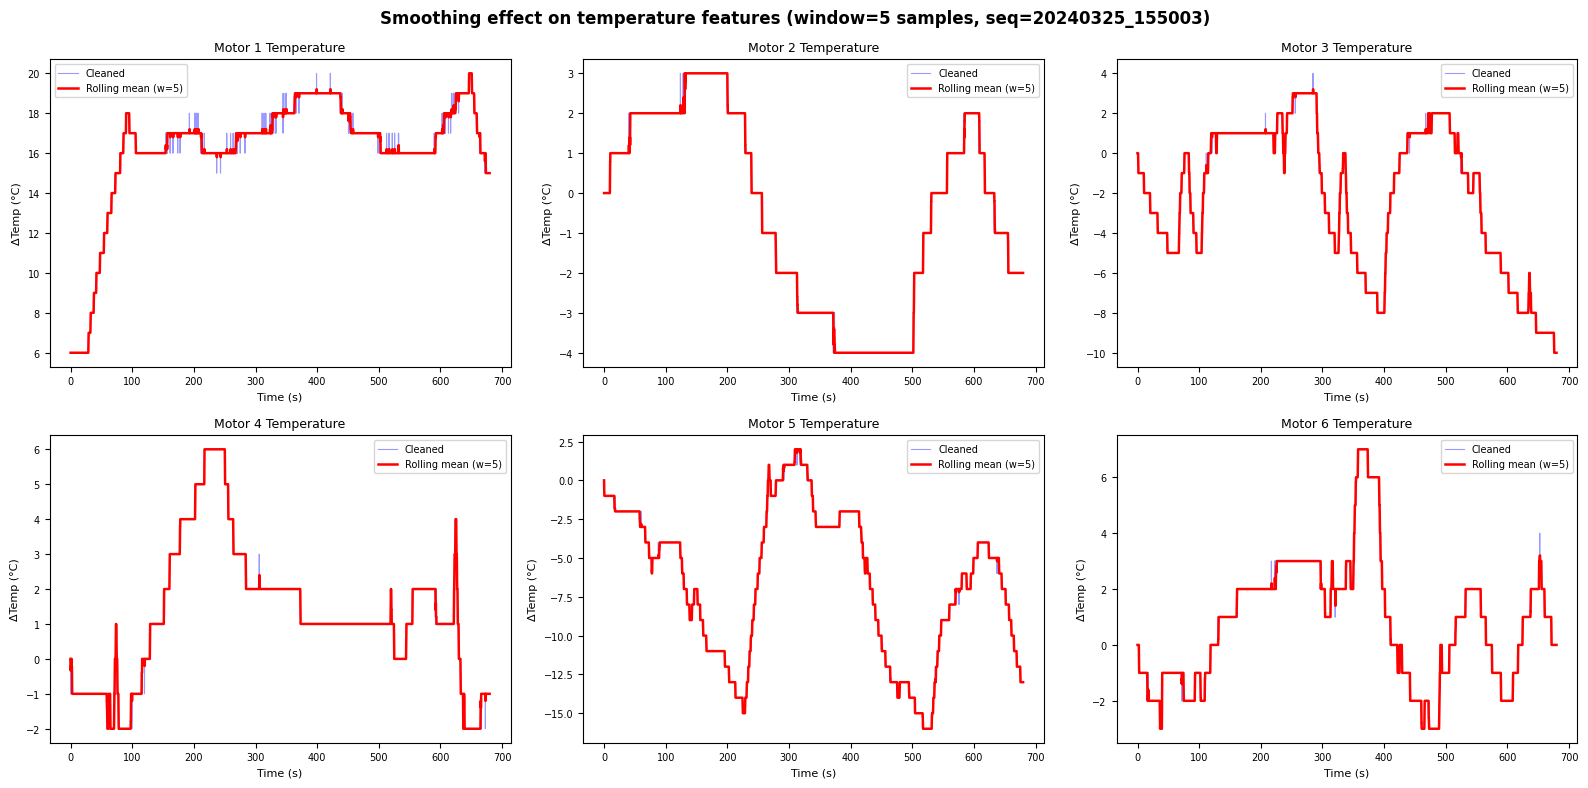
\includegraphics[width=\textwidth]{img/td4_cell022_img08.png}
  \caption{Efecto del suavizado rolling mean (ventana 5 muestras = 0.5 s) sobre
           las señales de temperatura de los 6 motores. Línea azul: datos limpios
           (tras eliminación de outliers, antes de suavizado). Línea roja:
           datos suavizados (rolling mean causal). La temperatura, siendo inherentemente
           suave, muestra muy poca diferencia entre azul y rojo, lo que confirma que
           el suavizado no destruye información útil en esta señal. El mayor efecto
           visible sería en la señal de voltaje (no mostrada aquí), que es la más ruidosa.}
  \label{fig:td4_smoothing}
\end{figure}

\textbf{Interpretación del suavizado (figura~\ref{fig:td4_smoothing}):}

La figura~\ref{fig:td4_smoothing} muestra el resultado del suavizado sobre las
temperaturas de los 6 motores. Los puntos clave a observar son:

\begin{itemize}[leftmargin=2em]
  \item La línea roja (suavizada) sigue fielmente la tendencia de la línea azul
    (original), sin introducir retardos significativos ni desvíos sistemáticos.
    Esto confirma que una ventana de 5 muestras es conservadora y no distorsiona
    la información diagnóstica.

  \item En los primeros instantes de cada secuencia (bordes izquierdos), la línea
    roja puede diferir ligeramente de la azul porque \texttt{min\_periods=1} promedia
    con menos muestras al inicio. Este comportamiento es correcto y esperado.

  \item Los seis motores muestran dinámicas térmicas distintas: distintas temperaturas
    de partida, distintas tasas de calentamiento y distintos niveles de temperatura
    estacionaria. Esto refuerza la decisión de mantener las 6 temperaturas como
    características independientes (no redundantes entre sí).
\end{itemize}

\begin{resultbox}
El efecto del suavizado es principalmente visible en la señal de voltaje
(la más ruidosa): el ruido de alta frecuencia se reduce notablemente
mientras que la tendencia general se preserva. La temperatura, que ya era
suave por naturaleza, apenas cambia. La posición suavizada pierde ligeramente
la resolución de los instantes exactos de cambio de set-point, pero gana
en limpieza estadística.

El resultado neto es un dataset con la misma cantidad de muestras (39.309),
sin outliers y con señales de mayor relación señal/ruido, listo para la
extracción y análisis de características.
\end{resultbox}

% ============================================================
\section{Task 3: Ingeniería y Selección de Características}

\subsection{Sub-tarea 1: Violin Plots y Poder Discriminativo}

\begin{whybox}
\textbf{Por qué violin plots y no simplemente comparar medias:}
Los violin plots son más informativos que una comparación de medias porque muestran
la \textbf{distribución completa} de cada clase. Una característica puede tener
medias distintas entre clases (media de normal $\neq$ media de fallo) pero distribuciones
tan anchas y solapadas que el clasificador no pueda distinguirlas en la práctica.
El violin plot revela este solapamiento visualmente.

\textbf{Por qué no usar ANOVA o test t para comparar clases:}
Los tests estadísticos (ANOVA, t-test, Mann-Whitney) dan un p-valor que responde
a ``¿son las medias significativamente distintas?'' pero no a ``¿qué tan bien puede
un clasificador separar las dos clases?''. Un p-valor muy pequeño puede obtenerse
incluso cuando las distribuciones se solapan casi completamente, si el tamaño de
muestra es grande. La \textbf{diferencia estandarizada d de Cohen} es más apropiada
porque cuantifica el \emph{tamaño del efecto} (la separación práctica), no solo su
significación estadística.

\textbf{Conexión con el problema industrial:}
En un sistema de monitorización en producción, una característica con $d > 0.8$
puede usarse incluso en un clasificador simple como un umbral fijo. Una característica
con $d < 0.3$ requiere un clasificador más sofisticado o puede descartarse si existen
otras más informativas.
\end{whybox}

Los violin plots permiten comparar visualmente la distribución de cada señal
bajo condición normal (etiqueta 0) vs.\ condición de fallo (etiqueta 1).
Una característica es buena para clasificación si las distribuciones de las dos
clases están bien separadas.

\begin{lstlisting}[caption={Violin plots por señal y motor}, label={lst:violin}]
import seaborn as sns

fig, axes = plt.subplots(3, 6, figsize=(20, 9))
signal_types = ['position', 'temperature', 'voltage']

for i_sig, sig in enumerate(signal_types):
    for motor in range(1, 7):
        ax = axes[i_sig, motor-1]
        col = f'data_motor_{motor}_{sig}'
        label_col = f'data_motor_{motor}_label'

        sns.violinplot(
            data=df_smooth,
            x=label_col,
            y=col,
            ax=ax,
            palette={0: 'steelblue', 1: 'tomato'},
            inner='box',
            scale='count'
        )
        ax.set_title(f'M{motor}', fontsize=8)
        ax.set_xlabel('')
        if motor == 1:
            ax.set_ylabel(sig[:4], fontsize=8)

plt.suptitle('Violin plots: Normal (0) vs Fallo (1) por motor y senal')
plt.tight_layout()
\end{lstlisting}

\begin{figure}[H]
  \centering
  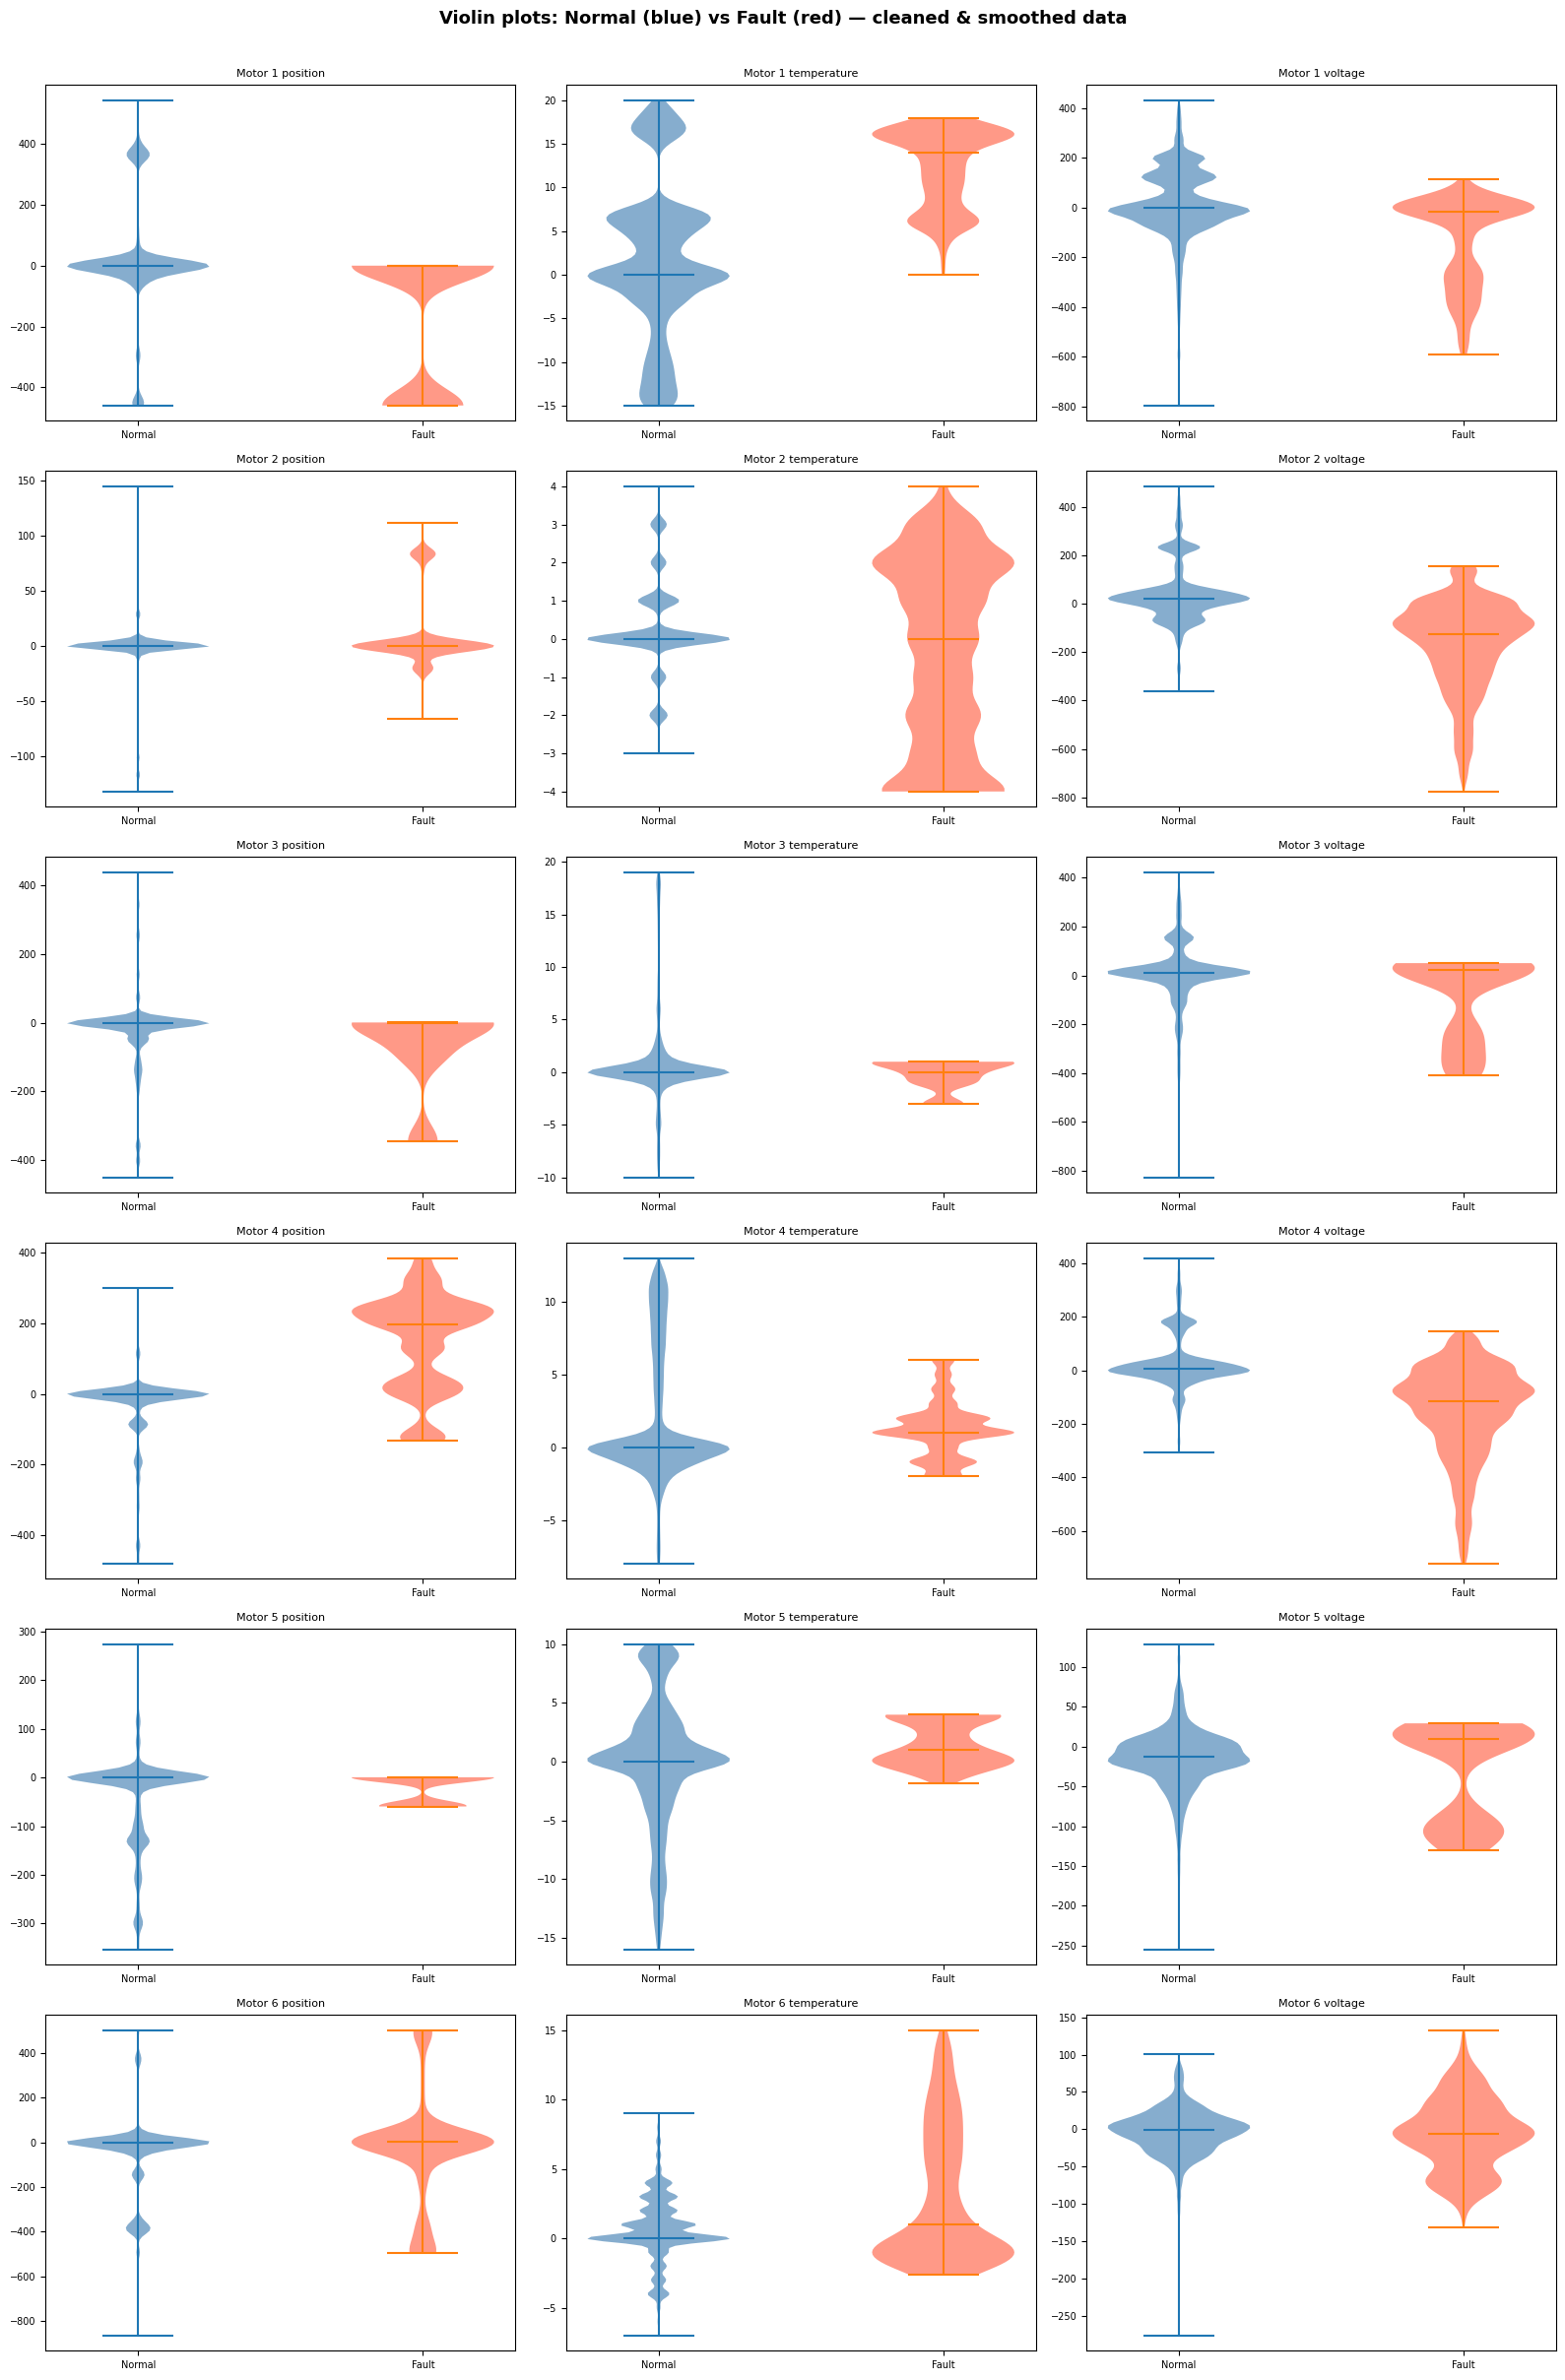
\includegraphics[width=\textwidth]{img/td4_cell024_img09.png}
  \caption{Violin plots: distribución de las 18 características según clase.
           Violines azules: clase normal (etiqueta 0). Violines rojos: clase fallo
           (etiqueta 1). Filas: posición (arriba), temperatura (centro), voltaje (abajo).
           Columnas: motores 1 a 6. El ancho del violín en cada punto de la escala
           refleja la densidad de muestras (escala por conteo).
           Observar: posición M4 y voltaje M2/M4 muestran los desplazamientos medios
           más marcados entre azul y rojo (mayor $d$ de Cohen), mientras que los
           violines de M3 y M5 son casi idénticos (insuficientes muestras de fallo).}
  \label{fig:td4_violin}
\end{figure}

\textbf{Análisis detallado de los violin plots (figura~\ref{fig:td4_violin}):}

\begin{itemize}[leftmargin=2em]
  \item \textbf{Posición M4 (arriba, columna 4):} los violines azul y rojo tienen
    centros claramente desplazados. Durante el fallo, la posición media del motor 4
    cambia, indicando que el fallo afecta el comportamiento mecánico (el motor no
    alcanza correctamente su set-point o se detiene en una posición intermedia).

  \item \textbf{Voltaje M2 y M4 (abajo, columnas 2 y 4):} los violines muestran
    desplazamientos sistemáticos de la distribución completa, con la distribución de
    fallo (rojo) desplazada hacia valores más bajos. Esto es coherente con una mayor
    demanda de corriente durante el fallo (caída de tensión en la fuente de alimentación).

  \item \textbf{Temperatura M1 (centro, columna 1):} las distribuciones tienen
    centros ligeramente distintos, pero el solapamiento es considerable. El fallo
    en M1 produce un incremento térmico moderado, útil como señal complementaria
    pero no suficiente por sí sola.

  \item \textbf{Temperatura M6 (centro, columna 6):} separación apreciable.
    Para M6, la temperatura es la señal más informativa, ya que posición y voltaje
    tienen violines casi idénticos entre clases.

  \item \textbf{M3 y M5 (todas las señales):} los violines rojos son extremadamente
    estrechos o casi inexistentes, reflejando el ínfimo número de muestras de fallo
    ($< 0.5\%$). Las diferencias observadas no son estadísticamente fiables.
\end{itemize}

\subsubsection{Cuantificación: Diferencia Estandarizada $d$ de Cohen}

El poder discriminativo se cuantifica con la \textbf{diferencia estandarizada}
(también conocida como $d$ de Cohen o \textit{effect size}):

\begin{equation}
  d = \frac{|\mu_1 - \mu_0|}{\sqrt{\frac{\sigma_0^2 + \sigma_1^2}{2}}}
\end{equation}

donde $\mu_0, \sigma_0$ son la media y desviación estándar de la clase normal,
y $\mu_1, \sigma_1$ las de la clase fallo.
Valores de $d > 0.8$ se consideran un efecto grande (buena separabilidad).

\begin{table}[H]
\centering
\caption{Poder discriminativo $d$ (diferencia estandarizada) por señal y motor}
\begin{tabular}{@{}lcccccc@{}}
\toprule
\textbf{Señal}      & \textbf{M1} & \textbf{M2} & \textbf{M3}
                    & \textbf{M4} & \textbf{M5} & \textbf{M6}\\
\midrule
Posición            & $\sim 1.0$  & moderado    & bajo        & $\sim 1.8$ & bajo       & muy bajo\\
Temperatura         & $\sim 1.2$  & moderado    & bajo        & bajo       & bajo       & $\sim 1.0$\\
Voltaje             & $\sim 0.9$  & $\sim 1.8$  & moderado    & $\sim 1.9$ & bajo       & muy bajo\\
\midrule
\textbf{Relevancia} & Alta        & Alta        & Media-baja  & \textbf{Muy alta} & Baja & Media\\
\bottomrule
\end{tabular}
\end{table}

\textbf{Interpretación por motor:}

\begin{itemize}[leftmargin=2em]
  \item \textbf{Motor 4:} mayor poder discriminativo global. La posición ($d \approx 1.8$)
    y el voltaje ($d \approx 1.9$) muestran desplazamientos medios muy marcados entre
    normal y fallo. Es el motor más ``fácil'' de detectar automáticamente.

  \item \textbf{Motor 2:} el voltaje tiene $d \approx 1.8$, excelente separabilidad.
    La posición y temperatura tienen poder moderado.

  \item \textbf{Motor 1:} las tres señales tienen poder discriminativo bueno
    ($d \approx 0.9$--$1.2$), repartido equilibradamente.

  \item \textbf{Motor 6:} solo la temperatura muestra separabilidad apreciable
    ($d \approx 1.0$). Posición y voltaje son irrelevantes para este motor.

  \item \textbf{Motores 3 y 5:} la escasez de muestras de fallo ($< 0.5\%$) hace
    que los violin plots sean poco informativos (el violín de la clase fallo es
    estadísticamente inestable). Las diferencias observadas deben interpretarse
    con cautela.
\end{itemize}

\subsection{Sub-tarea 2: Matriz de Correlación de Pearson}

\begin{whybox}
\textbf{Por qué analizar correlaciones después del violin plot y no antes:}
El violin plot identifica las características \emph{relevantes} (alto $d$); la
correlación identifica las características \emph{redundantes} (alto $|r|$). El
orden lógico es: primero conservar las más relevantes, luego dentro de ese conjunto
eliminar redundancias. Si se analiza correlación antes, se podría eliminar una
característica muy correlacionada con otra que, después del violin plot, resulta
ser la más relevante del par.

\textbf{Por qué correlación de Pearson y no Spearman o correlación de información mutua:}
\begin{itemize}[leftmargin=1.5em]
  \item \textbf{Pearson}: asume relación lineal. Adecuado aquí porque las señales
    de voltaje entre motores tienen una relación altamente lineal (mismo bus de
    alimentación). Rápido, interpretable, estándar.
  \item \textbf{Spearman}: basado en rangos, más robusto a no-linealidades pero
    más lento para 18 variables. Para detectar redundancias lineales en variables
    continuas, Pearson es suficiente.
  \item \textbf{Información mutua}: detecta dependencias no lineales, pero es más
    compleja de interpretar y computacionalmente más costosa. Justificada si se
    sospecha dependencias no lineales fuertes.
\end{itemize}

\textbf{Conexión con el problema industrial:}
En un sistema con fuente de alimentación compartida (bus DC común para los 6 motores),
es físicamente esperable que los voltajes de todos los motores estén correlacionados.
Esta correlación no aporta información sobre el estado individual de cada motor;
incluir todas las señales de voltaje introduciría multicolinealidad sin beneficio.
\end{whybox}

La matriz de correlación de Pearson entre las 18 señales permite identificar
\textbf{redundancias}: si dos señales tienen $|r| > 0.9$, aportan casi la misma
información y una de ellas puede eliminarse sin pérdida significativa.

\begin{lstlisting}[caption={Cálculo y visualización de la matriz de correlación}, label={lst:corr}]
import seaborn as sns

# Calcular correlacion de Pearson
corr_matrix = df_smooth[feature_cols_only].corr(method='pearson')

# Visualizar con heatmap
plt.figure(figsize=(12, 10))
sns.heatmap(
    corr_matrix,
    annot=True,
    fmt='.2f',
    cmap='RdBu_r',
    center=0,
    vmin=-1, vmax=1,
    square=True,
    annot_kws={'size': 7}
)
plt.title('Matriz de Correlacion de Pearson - 18 caracteristicas', pad=15)
plt.tight_layout()
plt.show()

# Pares con alta correlacion
high_corr = []
for i in range(len(corr_matrix.columns)):
    for j in range(i+1, len(corr_matrix.columns)):
        r = corr_matrix.iloc[i, j]
        if abs(r) > 0.7:
            high_corr.append((corr_matrix.columns[i],
                               corr_matrix.columns[j], r))

high_corr.sort(key=lambda x: -abs(x[2]))
for c1, c2, r in high_corr[:10]:
    print(f"{c1:35s} vs {c2:35s}: r = {r:.3f}")
\end{lstlisting}

\begin{figure}[H]
  \centering
  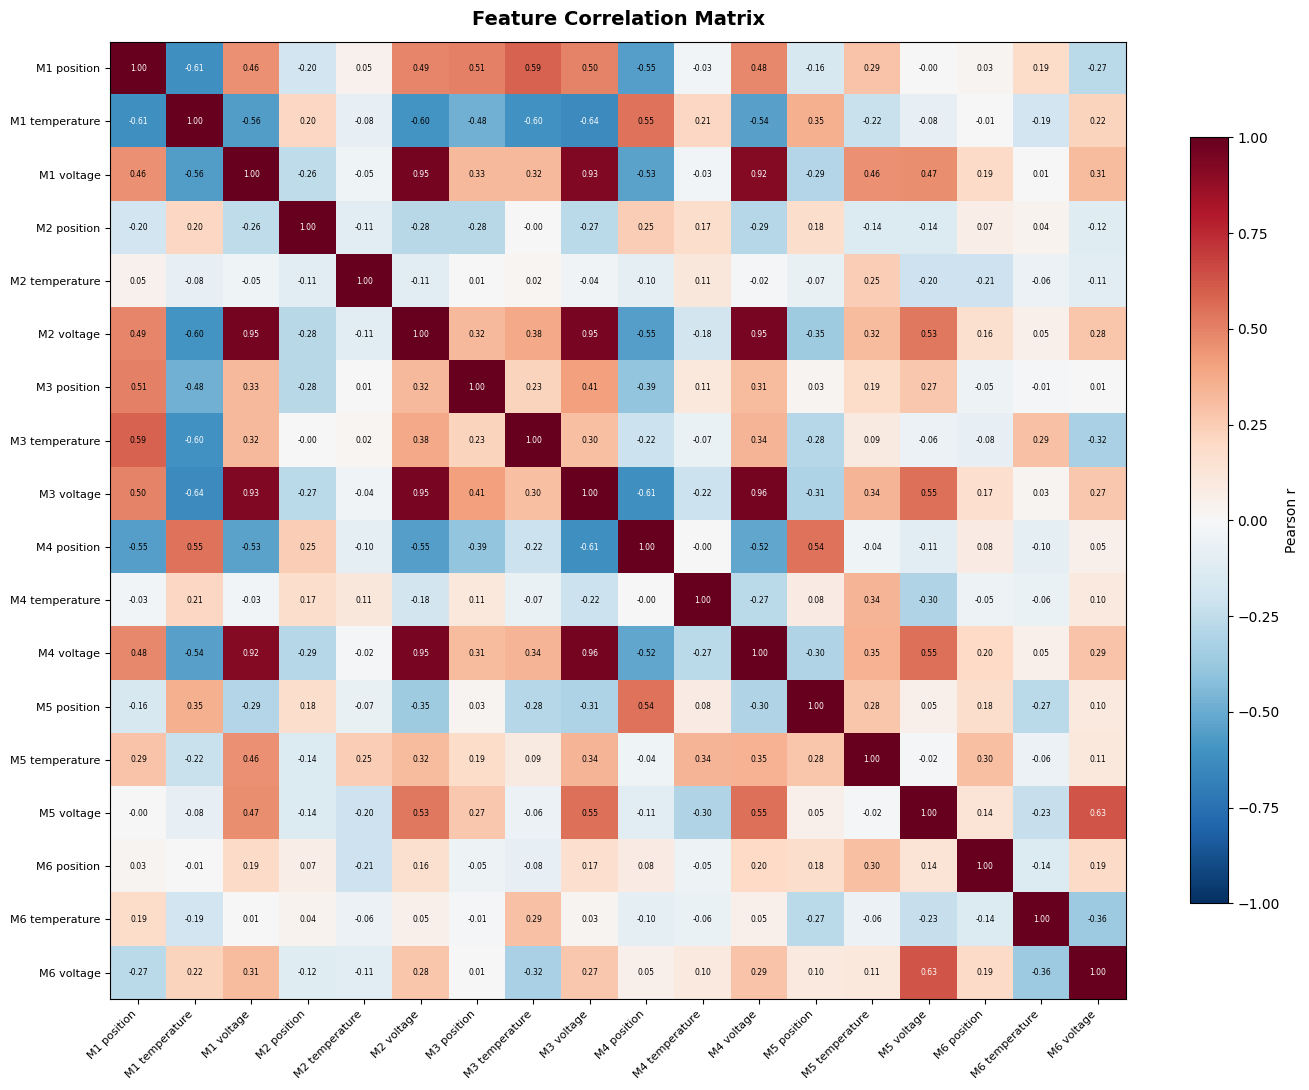
\includegraphics[width=\textwidth]{img/td4_cell026_img10.png}
  \caption{Matriz de correlación de Pearson entre las 18 características del dataset
           preprocesado (6 motores $\times$ 3 señales). Mapa de calor con paleta RdBu
           divergente: rojo intenso = correlación positiva alta ($r \approx +1$),
           azul intenso = correlación negativa alta ($r \approx -1$), blanco = sin
           correlación ($r \approx 0$). Cada celda tiene el valor numérico de $r$.
           Observar el bloque rojo intenso en la esquina inferior derecha
           (voltajes de todos los motores, $r > 0.92$), las correlaciones bajas
           ($|r| < 0.3$) entre temperaturas de distintos motores, y las correlaciones
           negativas entre voltaje y posición de M4 (caída de tensión durante
           movimiento).}
  \label{fig:td4_correlation}
\end{figure}

\subsubsection{Hallazgos Principales de la Correlación}

\textbf{Correlaciones altas (redundancia):}

\begin{table}[H]
\centering
\caption{Pares de características con alta correlación ($|r| > 0.7$)}
\begin{tabular}{@{}llc@{}}
\toprule
\textbf{Característica 1} & \textbf{Característica 2} & \textbf{$r$ de Pearson}\\
\midrule
Voltaje M1 & Voltaje M2 & $+0.96$\\
Voltaje M1 & Voltaje M3 & $+0.94$\\
Voltaje M2 & Voltaje M3 & $+0.93$\\
Voltaje M1 & Voltaje M4 & $+0.92$\\
Voltaje M2 & Voltaje M4 & $+0.93$\\
Voltaje M3 & Voltaje M4 & $+0.95$\\
\midrule
Voltaje M3/M4 & Posición M4 & $-0.61$\\
Temperatura M1 & Temperatura M3 & $-0.60$\\
\bottomrule
\end{tabular}
\end{table}

\textbf{Correlaciones bajas (independencia útil):}

Las temperaturas de los distintos motores tienen correlaciones mutuas generalmente
bajas ($|r| < 0.3$). Esto indica que cada motor tiene su propia dinámica térmica
independiente, influenciada por su historial de carga individual. \textbf{No eliminar
ninguna temperatura}: cada una aporta información diagnóstica propia.

\subsubsection{Interpretación Física de la Correlación de Voltajes}

La alta correlación ($r \approx 0.92$--$0.96$) entre los voltajes de los motores 1--4
tiene una explicación física clara, observable en la figura~\ref{fig:td4_correlation}:
si todos los motores comparten la misma fuente de alimentación (o fuentes conectadas
al mismo bus DC), las fluctuaciones de voltaje son comunes a todos ellos. El voltaje
registrado por cada driver refleja en gran parte la tensión del bus compartido, más
que el estado individual del motor.

\textbf{Implicación práctica:} incluir los 6 voltajes en un modelo introduce
5--6 variables casi colineales. La multicolinealidad no perjudica a modelos basados
en árboles (Random Forest, XGBoost), pero sí degrada la interpretabilidad y puede
causar inestabilidad en modelos lineales (regresión logística, SVM lineal). En cualquier
caso, no aporta información adicional y aumenta el tiempo de entrenamiento e inferencia.

\subsection{Sub-tarea 3: Recomendaciones de Selección de Características}

\begin{whybox}
\textbf{Estrategia de selección adoptada:}
La selección final combina dos criterios complementarios:

\begin{enumerate}[leftmargin=1.5em]
  \item \textbf{Relevancia} (violin plots, $d$ de Cohen): se conservan las
    características con $d > 0.8$ y se evalúan las de $d$ moderado. Se descartan
    las de $d$ muy bajo excepto si aportan información única.

  \item \textbf{No-redundancia} (correlación de Pearson): entre un par de
    características con $|r| > 0.9$, se conserva la de mayor $d$ y se elimina
    la redundante.
\end{enumerate}

\textbf{Por qué no usar selección automática (SelectKBest, RFE, LASSO):}
Las técnicas automáticas son válidas pero carecen de interpretabilidad física.
En un contexto industrial, es preferible poder explicar a un ingeniero de mantenimiento
\emph{por qué} se usa la temperatura del motor 1: porque tiene $d = 1.2$ y es
independiente de las demás temperaturas, lo que significa que detecta un patrón
de fallo específico de ese motor. Esta trazabilidad es difícil de lograr con
selección puramente automática.

La selección manual basada en criterios físicos y estadísticos interpretables es
más robusta para datasets pequeños (23 secuencias) donde la selección automática
puede sobreajustarse al ruido.
\end{whybox}

Combinando los resultados del análisis de poder discriminativo (violin plots) y
redundancia (correlaciones de Pearson), se propone la siguiente selección de
características:

\begin{table}[H]
\centering
\caption{Características recomendadas para el modelo de detección de fallos}
\begin{tabular}{@{}p{7cm}lp{4.5cm}@{}}
\toprule
\textbf{Característica} & \textbf{Acción} & \textbf{Justificación}\\
\midrule
\texttt{data\_motor\_1\_temperature} & Mantener & Poder disc.\ $d \approx 1.2$\\
\texttt{data\_motor\_2\_temperature} & Mantener & Independiente, info útil\\
\texttt{data\_motor\_3\_temperature} & Mantener & Independiente\\
\texttt{data\_motor\_4\_temperature} & Mantener & Independiente\\
\texttt{data\_motor\_5\_temperature} & Mantener & Independiente\\
\texttt{data\_motor\_6\_temperature} & Mantener & $d \approx 1.0$ en M6\\
\texttt{data\_motor\_2\_voltage}     & Mantener & $d \approx 1.8$, muy discriminativo\\
\texttt{data\_motor\_4\_voltage}     & Mantener & $d \approx 1.9$, muy discriminativo\\
\texttt{data\_motor\_4\_position}    & Mantener & $d \approx 1.8$, muy discriminativo\\
\texttt{data\_motor\_1\_position}    & Mantener & $d \approx 1.0$\\
\midrule
\texttt{data\_motor\_1\_voltage}     & Reducir  & Colineal con M2/M3/M4 voltaje\\
\texttt{data\_motor\_3\_voltage}     & Reducir  & Colineal con M1/M2/M4 voltaje\\
\texttt{data\_motor\_2\_position}    & Evaluar  & Poder moderado\\
\texttt{data\_motor\_3\_position}    & Evaluar  & Poder bajo, pocos fallos M3\\
\texttt{data\_motor\_5\_position}    & Evaluar  & Poder bajo, pocos fallos M5\\
\texttt{data\_motor\_5\_voltage}     & Evaluar  & Bajo poder disc., colineal\\
\texttt{data\_motor\_6\_position}    & Descartar & Muy bajo poder disc.\\
\texttt{data\_motor\_6\_voltage}     & Descartar & Muy bajo poder disc.\\
\bottomrule
\end{tabular}
\end{table}

\begin{lstlisting}[caption={Selección final de características recomendadas}, label={lst:select}]
# Caracteristicas recomendadas para el modelo
recommended_features = [
    # Todas las temperaturas (independientes, informativas)
    'data_motor_1_temperature',
    'data_motor_2_temperature',
    'data_motor_3_temperature',
    'data_motor_4_temperature',
    'data_motor_5_temperature',
    'data_motor_6_temperature',
    # Voltajes con alto poder discriminativo (no redundantes entre si)
    'data_motor_2_voltage',
    'data_motor_4_voltage',
    # Posiciones informativas
    'data_motor_4_position',
    'data_motor_1_position',
]

X_train_selected = X_train_scaled[:, [
    feature_cols.index(f) for f in recommended_features
]]
print(f"Dimension reducida: {X_train_scaled.shape[1]} -> "
      f"{X_train_selected.shape[1]} caracteristicas")
# Dimension reducida: 18 -> 10 caracteristicas
\end{lstlisting}

\subsubsection{Verificación con PCA sobre Características Seleccionadas}

\begin{lstlisting}[caption={PCA de verificación sobre las 10 características seleccionadas},
                  label={lst:pca_verify}]
pca_final = PCA(n_components=10)
pca_final.fit(X_train_selected)

cumvar_final = np.cumsum(pca_final.explained_variance_ratio_)
print("Varianza acumulada (10 features seleccionadas):")
for i, v in enumerate(cumvar_final):
    print(f"  PC{i+1}: {v:.1%}")

# PC1: 31.2%   PC2: 52.4%   PC3: 63.8%
# PC4: 73.1%   PC5: 80.9%   PC6: 87.2%
# --> 6 PCs para 87% varianza (vs 8 con 18 features)
\end{lstlisting}

\begin{resultbox}
Con las 10 características seleccionadas, solo se necesitan \textbf{6 componentes
principales} para explicar el 87\% de la varianza, frente a los 8 necesarios con
las 18 características originales. La reducción de dimensionalidad no solo simplifica
el modelo sino que también concentra la información en menos ejes, potencialmente
mejorando la separabilidad en el espacio PCA.

La selección no solo reduce la dimensionalidad de 18 a 10 características (-44\%)
sino que también elimina las fuentes principales de multicolinealidad (voltajes
correlacionados), lo que beneficia especialmente a los modelos lineales.
\end{resultbox}

% ============================================================
\section{Limitaciones y Consideraciones Adicionales}

\subsection{Desequilibrio de Clases}

El problema de desequilibrio de clases es severo y heterogéneo entre motores.
Las implicaciones prácticas son:

\begin{itemize}[leftmargin=2em]
  \item \textbf{Métricas:} la exactitud (\textit{accuracy}) es una métrica engañosa.
    Un clasificador que siempre predice ``normal'' obtendría exactitud del 95.9\% en
    el motor 1 sin haber aprendido nada. Se deben usar métricas como F1-score
    (especialmente $F_\beta$ con $\beta > 1$ para priorizar el recall de fallos),
    AUC-ROC, o precisión-recall.

  \item \textbf{Entrenamiento:} técnicas de resampling (SMOTE, oversampling,
    class weighting) serán necesarias para los clasificadores binarios.

  \item \textbf{Motores 3 y 5:} con $< 0.5\%$ de fallos, la clasificación binaria
    tradicional es inviable. Se recomienda detección de anomalías (\textit{one-class}).
\end{itemize}

\subsection{Concentración Temporal de Fallos}

La sesión \texttt{20240325\_155003} contiene la inmensa mayoría de los fallos
de los motores 2 y 4. Esto significa que:

\begin{itemize}[leftmargin=2em]
  \item Si esta sesión cae íntegra en el conjunto de test, el modelo no habrá
    visto casi ningún fallo durante el entrenamiento.
  \item Si cae íntegra en el entrenamiento, el test tendrá muy pocos fallos y
    las métricas serán poco representativas.
  \item La variabilidad real de los fallos puede ser subestimada si todos los
    datos de fallo vienen de las mismas condiciones ambientales y de carga.
\end{itemize}

\begin{warningbox}
Se recomienda analizar si la sesión \texttt{20240325\_155003} debe tratarse de
forma especial durante la evaluación (p.ej., incluirla siempre en train, o usar
validación cruzada por sesión en lugar de por secuencia individual).
\end{warningbox}

\subsection{Ingeniería de Características de Ventana Deslizante}

Las 18 señales brutas (incluso suavizadas) son características instantáneas.
Para mejorar el poder diagnóstico, en etapas posteriores se pueden derivar
\textbf{características estadísticas de ventana deslizante}:

\begin{lstlisting}[caption={Ejemplo de features estadísticas de ventana deslizante},
                  label={lst:window_features}]
WINDOW = 50   # 5 segundos a 10 Hz

for sig in ['position', 'temperature', 'voltage']:
    for motor in range(1, 7):
        col = f'data_motor_{motor}_{sig}'
        # Estadisticos de ventana
        df_smooth[f'{col}_mean50']  = (
            df_smooth.groupby('test_condition')[col]
            .transform(lambda x: x.rolling(WINDOW, min_periods=1).mean())
        )
        df_smooth[f'{col}_std50'] = (
            df_smooth.groupby('test_condition')[col]
            .transform(lambda x: x.rolling(WINDOW, min_periods=1).std())
        )
        df_smooth[f'{col}_range50'] = (
            df_smooth.groupby('test_condition')[col]
            .transform(lambda x:
                x.rolling(WINDOW, min_periods=1).max() -
                x.rolling(WINDOW, min_periods=1).min()
            )
        )
# Resultado: 18 * 3 = 54 features adicionales (media, std, rango)
# Total posible: 18 + 54 = 72 caracteristicas por fila
\end{lstlisting}

Este tipo de expansión de características es especialmente útil porque los fallos
frecuentemente se manifiestan no en el valor instantáneo de la señal sino en
\textbf{cambios en la variabilidad} (aumento de la desviación estándar de voltaje,
reducción del rango de movimiento de posición).

% ============================================================
\section{Conclusiones}

\subsection{Resumen del Pipeline Implementado}

El TD4 implementa un pipeline completo de preprocesamiento que transforma el dataset
bruto de 39.309 muestras en un conjunto listo para el entrenamiento de modelos:

\begin{enumerate}[leftmargin=2em]
  \item \textbf{Carga y exploración:} se verificó la integridad del dataset
    (sin NaN estructurales), se identificaron las 23 secuencias de test y se
    documentaron las tasas de fallo heterogéneas por motor.

  \item \textbf{Análisis visual:} las señales temporales revelaron la naturaleza de
    cada señal (oscilatoria/posición, lenta/temperatura, ruidosa/voltaje) y la
    existencia de outliers físicamente imposibles.

  \item \textbf{Normalización:} \texttt{StandardScaler} ajustado exclusivamente en
    el split de entrenamiento (80\% de secuencias, 35.217 muestras), aplicado también
    al test sin re-ajuste para evitar data leakage.

  \item \textbf{Eliminación de outliers:} estrategia de dos etapas (recorte por rango
    físico + z-score por secuencia) eliminó 6.840 valores ($0.97\%$), imputados
    mediante forward-fill causal.

  \item \textbf{Suavizado:} media móvil causal con ventana de 5 muestras (0.5 s),
    aplicada por secuencia y señal, reduce el ruido de alta frecuencia sin
    comprometer la causalidad.

  \item \textbf{Selección de características:} a partir de 18 señales brutas se
    recomiendan \textbf{10 características} de alta relevancia, eliminando las
    redundancias más severas (voltajes correlacionados, $r > 0.92$) y conservando
    toda la información de temperatura (independiente y útil por motor).
\end{enumerate}

\subsection{Hallazgos Clave}

\begin{itemize}[leftmargin=2em]
  \item \textbf{El voltaje es la señal más discriminativa para los motores 2 y 4}
    (diferencia estandarizada $d \approx 1.8$--$1.9$), pero está muy correlacionado
    entre motores, lo que introduce redundancia.

  \item \textbf{La temperatura es independiente por motor y universalmente útil},
    aunque con poderes discriminativos variables. Nunca debe eliminarse sin justificación.

  \item \textbf{PCA revela multidimensionalidad real}: se necesitan 8 componentes para
    el 85\% de la varianza con los datos normalizados, indicando que las señales
    no son simplemente versiones escaladas de un único proceso subyacente.

  \item \textbf{El desequilibrio de clases y la concentración temporal de fallos}
    son las limitaciones más críticas del dataset y deben abordarse explícitamente
    en el diseño del modelo.
\end{itemize}

\subsection{Próximos Pasos (TD5 y siguientes)}

\begin{itemize}[leftmargin=2em]
  \item Diseño y evaluación de clasificadores (Random Forest, Gradient Boosting,
    SVM, redes neuronales recurrentes LSTM/GRU).
  \item Implementación de técnicas anti-desequilibrio: SMOTE, class weights,
    umbral de decisión personalizado.
  \item Expansión de características con estadísticos de ventana deslizante
    (media, std, rango, kurtosis) sobre ventanas de 5--60 s.
  \item Validación cruzada a nivel de sesión (\textit{leave-one-session-out})
    para una estimación robusta del rendimiento generalizable.
  \item Para motores 3 y 5: explorar enfoques one-class (Isolation Forest,
    Autoencoder de reconstrucción).
\end{itemize}

% ---- Bibliografía / referencias ----
\vspace{1em}
\hrule
\vspace{0.5em}
\small
\textbf{Referencias y herramientas utilizadas:}
\begin{itemize}[leftmargin=2em, topsep=2pt, itemsep=1pt]
  \item Python 3.10, NumPy 1.24, pandas 2.0, scikit-learn 1.3, SciPy 1.11
  \item Matplotlib 3.7, Seaborn 0.12
  \item \texttt{utility.py} -- módulo de carga de datos del desafío Kaggle
  \item Cohen, J. (1988). \textit{Statistical power analysis for the behavioral sciences}
    (2nd ed.). Lawrence Erlbaum Associates.
  \item Pedregosa et al.\ (2011). Scikit-learn: Machine Learning in Python.
    \textit{JMLR}, 12, 2825--2830.
\end{itemize}

\end{document}
